\chapter{Anharmonischer Oszillator\label{chapter:anharmonisch}}
\lhead{Anharmonischer Oszillator}
\begin{refsection}
\chapterauthor{Joel Brunner und Christian Cavegn}

\newpage
			%Einleitung
\section{Einleitung}
\rhead{Einleitung}
In diesem Kapitel erweitern wir den harmonischen Oszillator aus Kapitel~\ref{chapter:harmonischeroszillator} mit Hilfe der St"orungstheorie aus Kapitel~\ref{chapter:stoerungstheorie}. Der harmonische Oszillator ist eine gute Approximation f"ur viele Quantenmechanische Systeme. Will man die Approximation verbessern, kann man die Kr"afte im Oszillator nicht mehr linear modellieren. Das Potential ist also nicht mehr nur $Q^2$, sondern es kommen noch Terme h"oherer Ordnung hinzu. Diese Terme k"onnen als St"orungen betrachtet werden. In diesem Kapitel sprechen wir oft von ungest"ort und gest"ort sowie von harmonisch und anharmonisch. Diese bedeuten in unserem Kontext das selbe.

\begin{figure}[h]	%Bild Titelbild.png
\centering
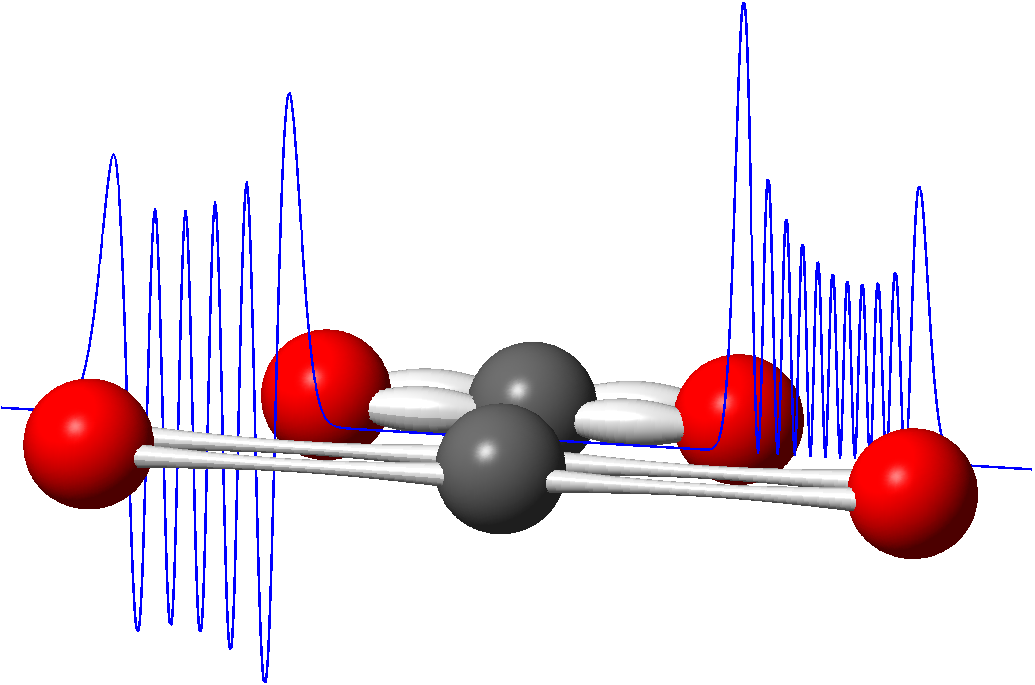
\includegraphics[width=0.7\textwidth]{anharmonisch/images/Titelbild.png}
\caption{Kohlendioxid Molek"ul
\label{skript:Titelbild}}
\end{figure}

			%Anharmonizität
\section{Anharmonizit"at}
\rhead{Anharmonizit"at}

\begin{figure}[h]	%Bild Potentiale
\centering
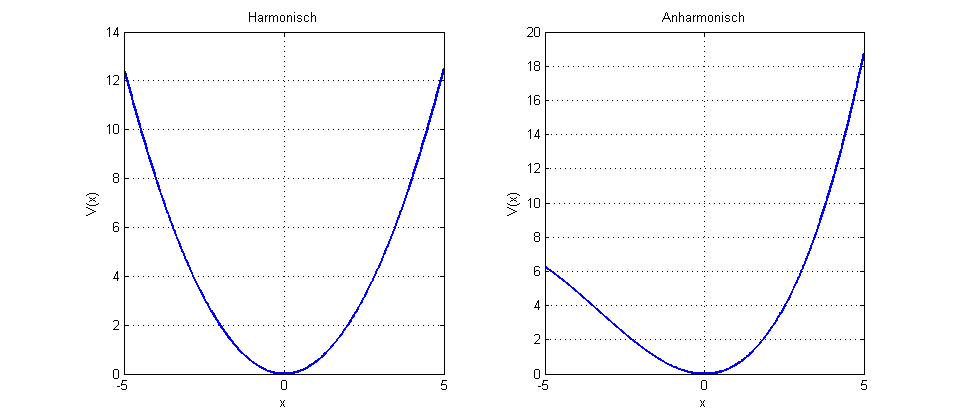
\includegraphics[width=0.7\textwidth]{anharmonisch/images/Potential.png}
\caption{Potentiale eines harmonischen und anharmonischen Oszillators
\label{skript:Potentiale}}
\end{figure}

Auf der Abbildung~\ref{skript:Potentiale} sieht man links das Potential des harmonischen Oszillators. Das System ist linear und wurde in Kapitel~\ref{chapter:harmonischeroszillator} vollst"andig gel"ost. Rechts sieht man das Potential des gest"orten Oszillators. In diesem Fall sind zus"atzlich noch Terme wie $aQ^3$ oder $bQ^4$ im Potential enhalten. Der harmonische Term ist aber immer noch der dominierende.

			%Harmonische Grössen
\section{Harmonische Gr"ossen}
\rhead{Harmonische Gr"ossen}

\begin{figure}[h]	%Bild Harmonisch.pdf
\centering
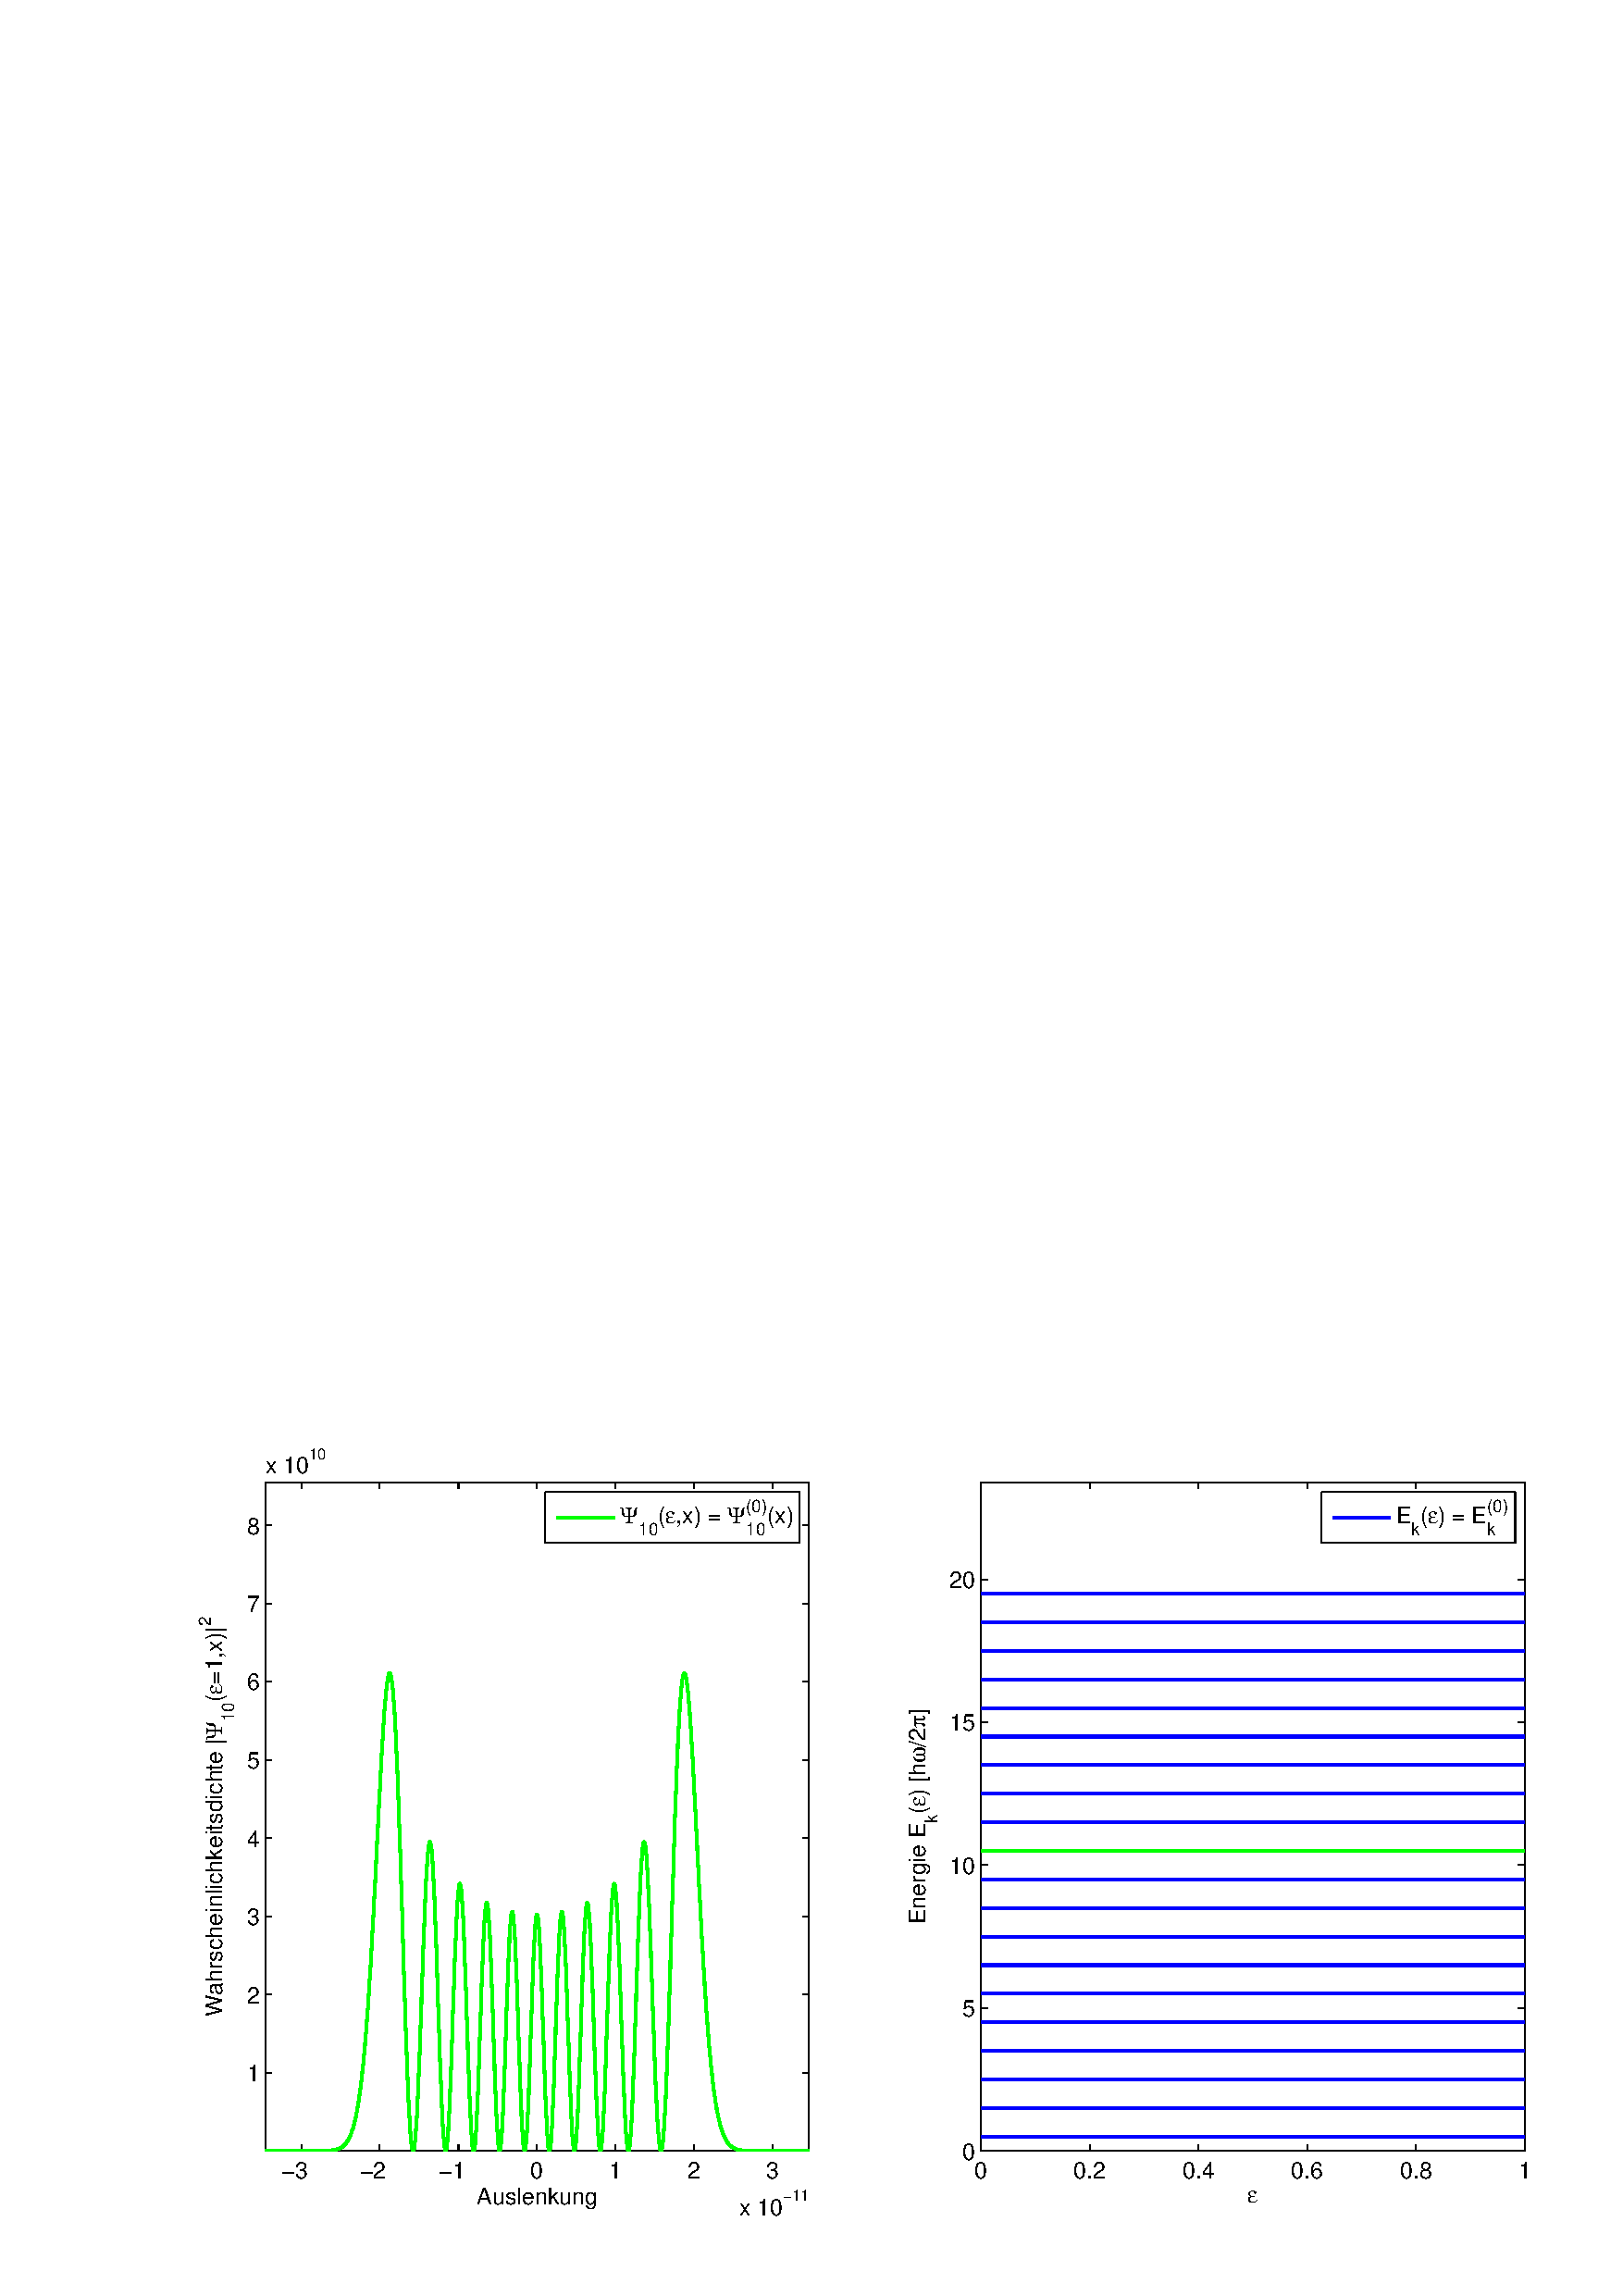
\includegraphics[width=0.7\textwidth]{anharmonisch/images/Harmonisch.pdf}
\caption{10. Wellenfunktion und Energieniveaus des harmonischen Oszillators
\label{skript:Harmonisch}}
\end{figure}

			%Wellenfunktionen
\subsection{Wellenfunktionen}
Der Grundzustand (\ref{skript:grundzustandwellenfunktion}) hat die Form einer Gauss-Kurve. Mit der geeigneten Normierung bekommen wir den Grundzustand
\[
\Psi_0(x)
=
\biggl(\frac{m\omega}{\pi\hbar}\biggr)^\frac14
e^{-\frac12\frac{m\omega}{\hbar}x^2}
\]
Aus der Gleichung
\[
|n\rangle
=
\frac{1}{\sqrt{N_n}}(a^+)^n\,|0\rangle
=
2^n \sqrt{\frac{n!}{2n!}} (a^+)^n\,|0\rangle
\]
wird eine eingache Iterationsfunktion Abgeleitet.
\[
\Psi_k(x)
=
\frac1{\sqrt{k!}}\biggl(\frac1{\sqrt{2}}
\biggl(\sqrt{\frac{m\omega}{\hbar}x}-
\sqrt{\frac{\hbar}{m\omega}}\frac{\partial}{\partial x}\biggr)\biggr)^k
\biggl(\frac{m\omega}{\pi\hbar}\biggr)^\frac14
e^{-\frac12\frac{m\omega}{\hbar}x^2}
\]
In die Gleichung substituiert man
\[
\alpha=\sqrt{\frac{m\omega}\hbar}
\]
und formt sie ein wenig um.
\[
\Psi_k(x)
=
\frac1{\sqrt{k!}}\frac1{\sqrt{2^k}}
\biggl(\frac{m\omega}{\pi\hbar}\biggr)^\frac14
\biggl(\alpha x-\frac1{\alpha}\frac{\partial}{\partial x}\biggr)^k
e^{-\frac12\alpha^2x^2}
\]
Durch ausmultiplizieren erhaltet man die entsprechende Wellenfunktion
\begin{align*}
\biggl(\alpha x-\frac1{\alpha}\frac{\partial}{\partial x}\biggr)^1
e^{-\frac12\alpha^2x^2}
&=
(2\alpha x)e^{-\frac12\alpha^2x^2}
\\
\biggl(\alpha x-\frac1{\alpha}\frac{\partial}{\partial x}\biggr)^2
e^{-\frac12\alpha^2x^2}
&=
\biggl(\alpha x-\frac1{\alpha}\frac{\partial}{\partial x}\biggr)
(2\alpha x)e^{-\frac12\alpha^2x^2}
\\
&=
\biggl(2\alpha^2 x^2-2\frac{\partial}{\partial x}x\biggr)
e^{-\frac12\alpha^2x^2}
\\
(2\alpha^2x^2-(2-2\alpha^2x^2))e^{-\frac12\alpha^2x^2}
&=
(4\alpha^2x^2-2)e^{-\frac12\alpha^2x^2}
\end{align*}
Man erh"alt die charakteristischen Hermitpolynome $H_k$, welche wir mit folgender Gleichung erhalten werden k"onnen. Dabei ist $z=ax$.
\[
H_k(z)
=
e^{\frac{z^2}2}\biggl(z-\frac{\partial}{\partial z}\biggr)^k
e^{-\frac{z^2}2}.
\]
Dadurch wird die Gleichung gek"urzt zu
\[
\Psi_k(z)
=
\biggl(\frac{m\omega}{\pi\hbar}\biggr)^\frac14
\frac1{\sqrt{2^k k!}}H_k(z)
e^{-\frac12 z^2}
\]

Der Vorteil dieser Notation ist die sehr einfache Implementierung in den g"angigen Berechunugstools

			%Energieniveaus			
\subsection{Energieniveaus}
\[
E_n
=
\hbar\omega\biggl(n+\frac12\biggr)
\]

			%Störungstheorie
\section{St"orungstheorie}
\rhead{St"orungstheorie}
Schr"odingergleichung in der St"orungstheorie
\[
(H_0+\varepsilon H_1)|\Psi_k(\varepsilon)\rangle
=
E_k(\varepsilon)|\Psi_k(\varepsilon)\rangle
\]
Koeffizienten
\begin{align*}
E_k(\varepsilon)
&=
E_k^{(0)}+\varepsilon E_k^{(1)}+\varepsilon^2 E_k^{(2)}+\dotsb
\\
|\Psi_k(\varepsilon)\rangle
&=
|\Psi_k^{(0)}\rangle+\varepsilon|\Psi_k^{(1)}\rangle+
\varepsilon^2|\Psi_k^{(2)}\rangle+\dotsb
\end{align*}
Durch geeignetes ausmultiplizieren wie in \ref{section:nichtentartetezustaende}  beschrieben kommt man auf folgende generische Gleichung:
\begin{align*}
\langle\Psi_l^{(0)}|\Psi_k^{(p)}\rangle
&=
\frac{C_{lk}^{p}-\langle\Psi_l^{(0)}|H_1|\Psi_k^{(k)}\rangle}
{E_l^{(0)}-E_k^{(0)}}
\\
E_k^{(p)}
&=
\langle\Psi_l^{(0)}|H_1|\Psi_l^{(k)}\rangle-C_{lk}^{(p)}
\end{align*}
mit
\[
C_{lk}^{(p)}
=
\displaystyle\sum_{j=2}^{p} E_k^{(p-j-1)}
\langle\Psi_l^{(0)}|\Psi_k^{(j-1)}\rangle
\]
Diese k"onnen einfach Implementiert werden\\
Code TODO\\
\\
Das Skalarprodukt beschreibt die Abh"angigkeit zweier Vektoren. Um sich eine bessere Vorstellung zu verschaffen dient folgende Gleichung
\[
|\langle\Psi_l^{(0)}|\Psi_k^{(p)}\rangle|^2
=
P(\Psi_l^{(0)}|\Psi_l^{(p)})
\]
Wie Wahrscheinlich ist es, dass die ungest"orte Wellenfunktion $|\Psi_l^{(0)}\rangle$ in der Zustandskorrektur $|\Psi_k^{(p)}\rangle$ vorkommt.

\[
\Psi_k^{(p)}
=
\imath\gamma|\Psi_l^{(0)}\rangle+
\displaystyle\sum_{l\neq k} \langle\Psi_l^{(0)}|\Psi_k^{(p)}\rangle
|\Psi_l^{(0)}\rangle
\]
			%Auswertung
\section{Auswertung}
\rhead{Auswertung}

Wir haben den Fall $aQ^3$ und $bQ^4$ mit Matlab durchgerechnet und sind auf ein Paar interessante Erkenntnisse gestossen. Auf den folgenden Abbildungen ist die stellen die Farbe gr"un immer den ungest"orten Fall dar und rot den gest"orten.

			%Erstes Beispiel
\subsection{Erstes Beispiel $aQ^3$}

\begin{figure}[h]	%Bild EK1.pdf
\centering
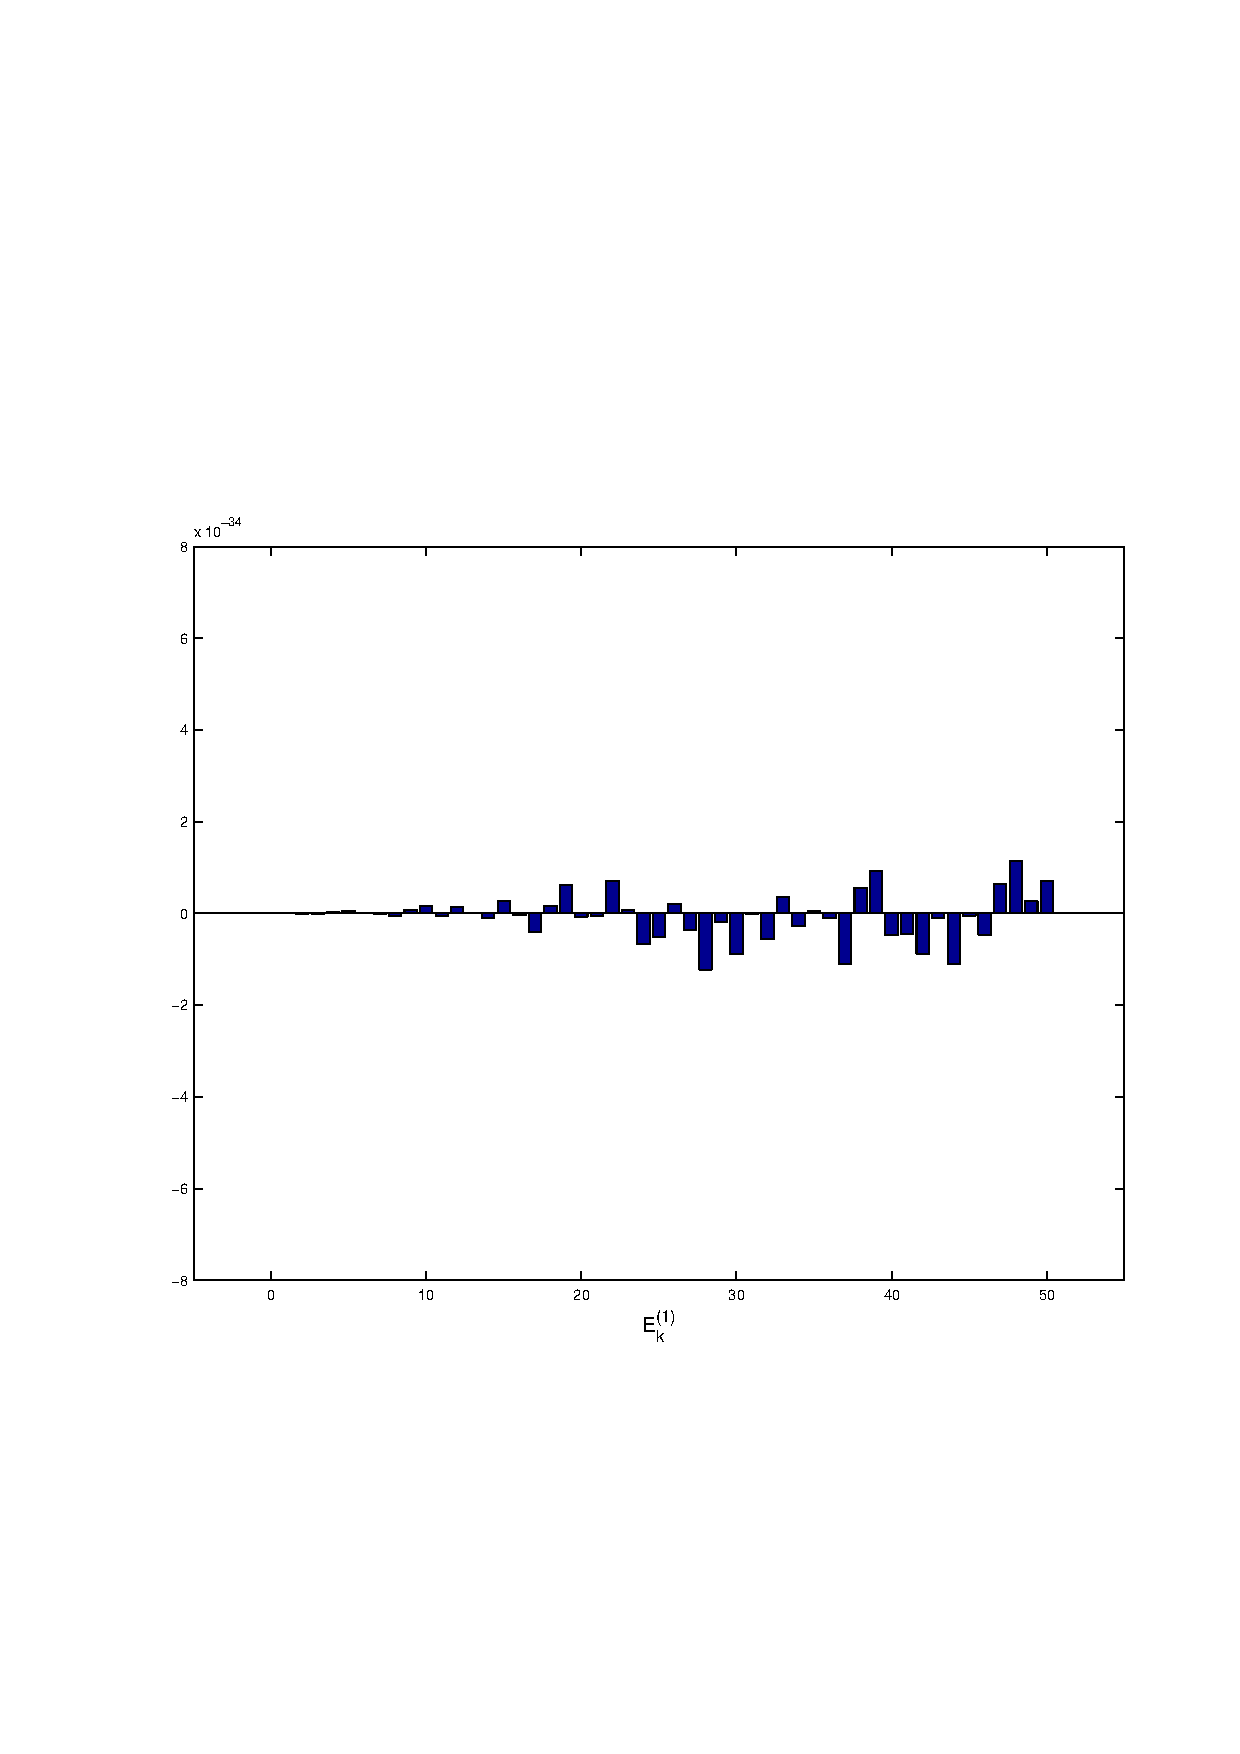
\includegraphics[width=0.6\textwidth]{anharmonisch/images/x3/EK1.pdf}
\caption{St"orung der Energieniveaus erster N"aherung
\label{skript:x3_EK1}}
\end{figure}

Auf der Abbildung~\ref{skript:x3_EK1} sieht man die "Anderung der Energieniveaus in erster N"aherung. Da die "Anderungen so klein sind k"onnen sie auf die numerische Berechnug mit Matlab zur"uckgef"uhrt werden. Wenn man die Gleichung~\ref{skript:stoerungsloesung1ordnung} genau betrachtet sieht man auch, dass die "Anderung Null sein muss.

\begin{figure}[h]	%Bild Stoerung1Wellenfunktion.pdf
\centering
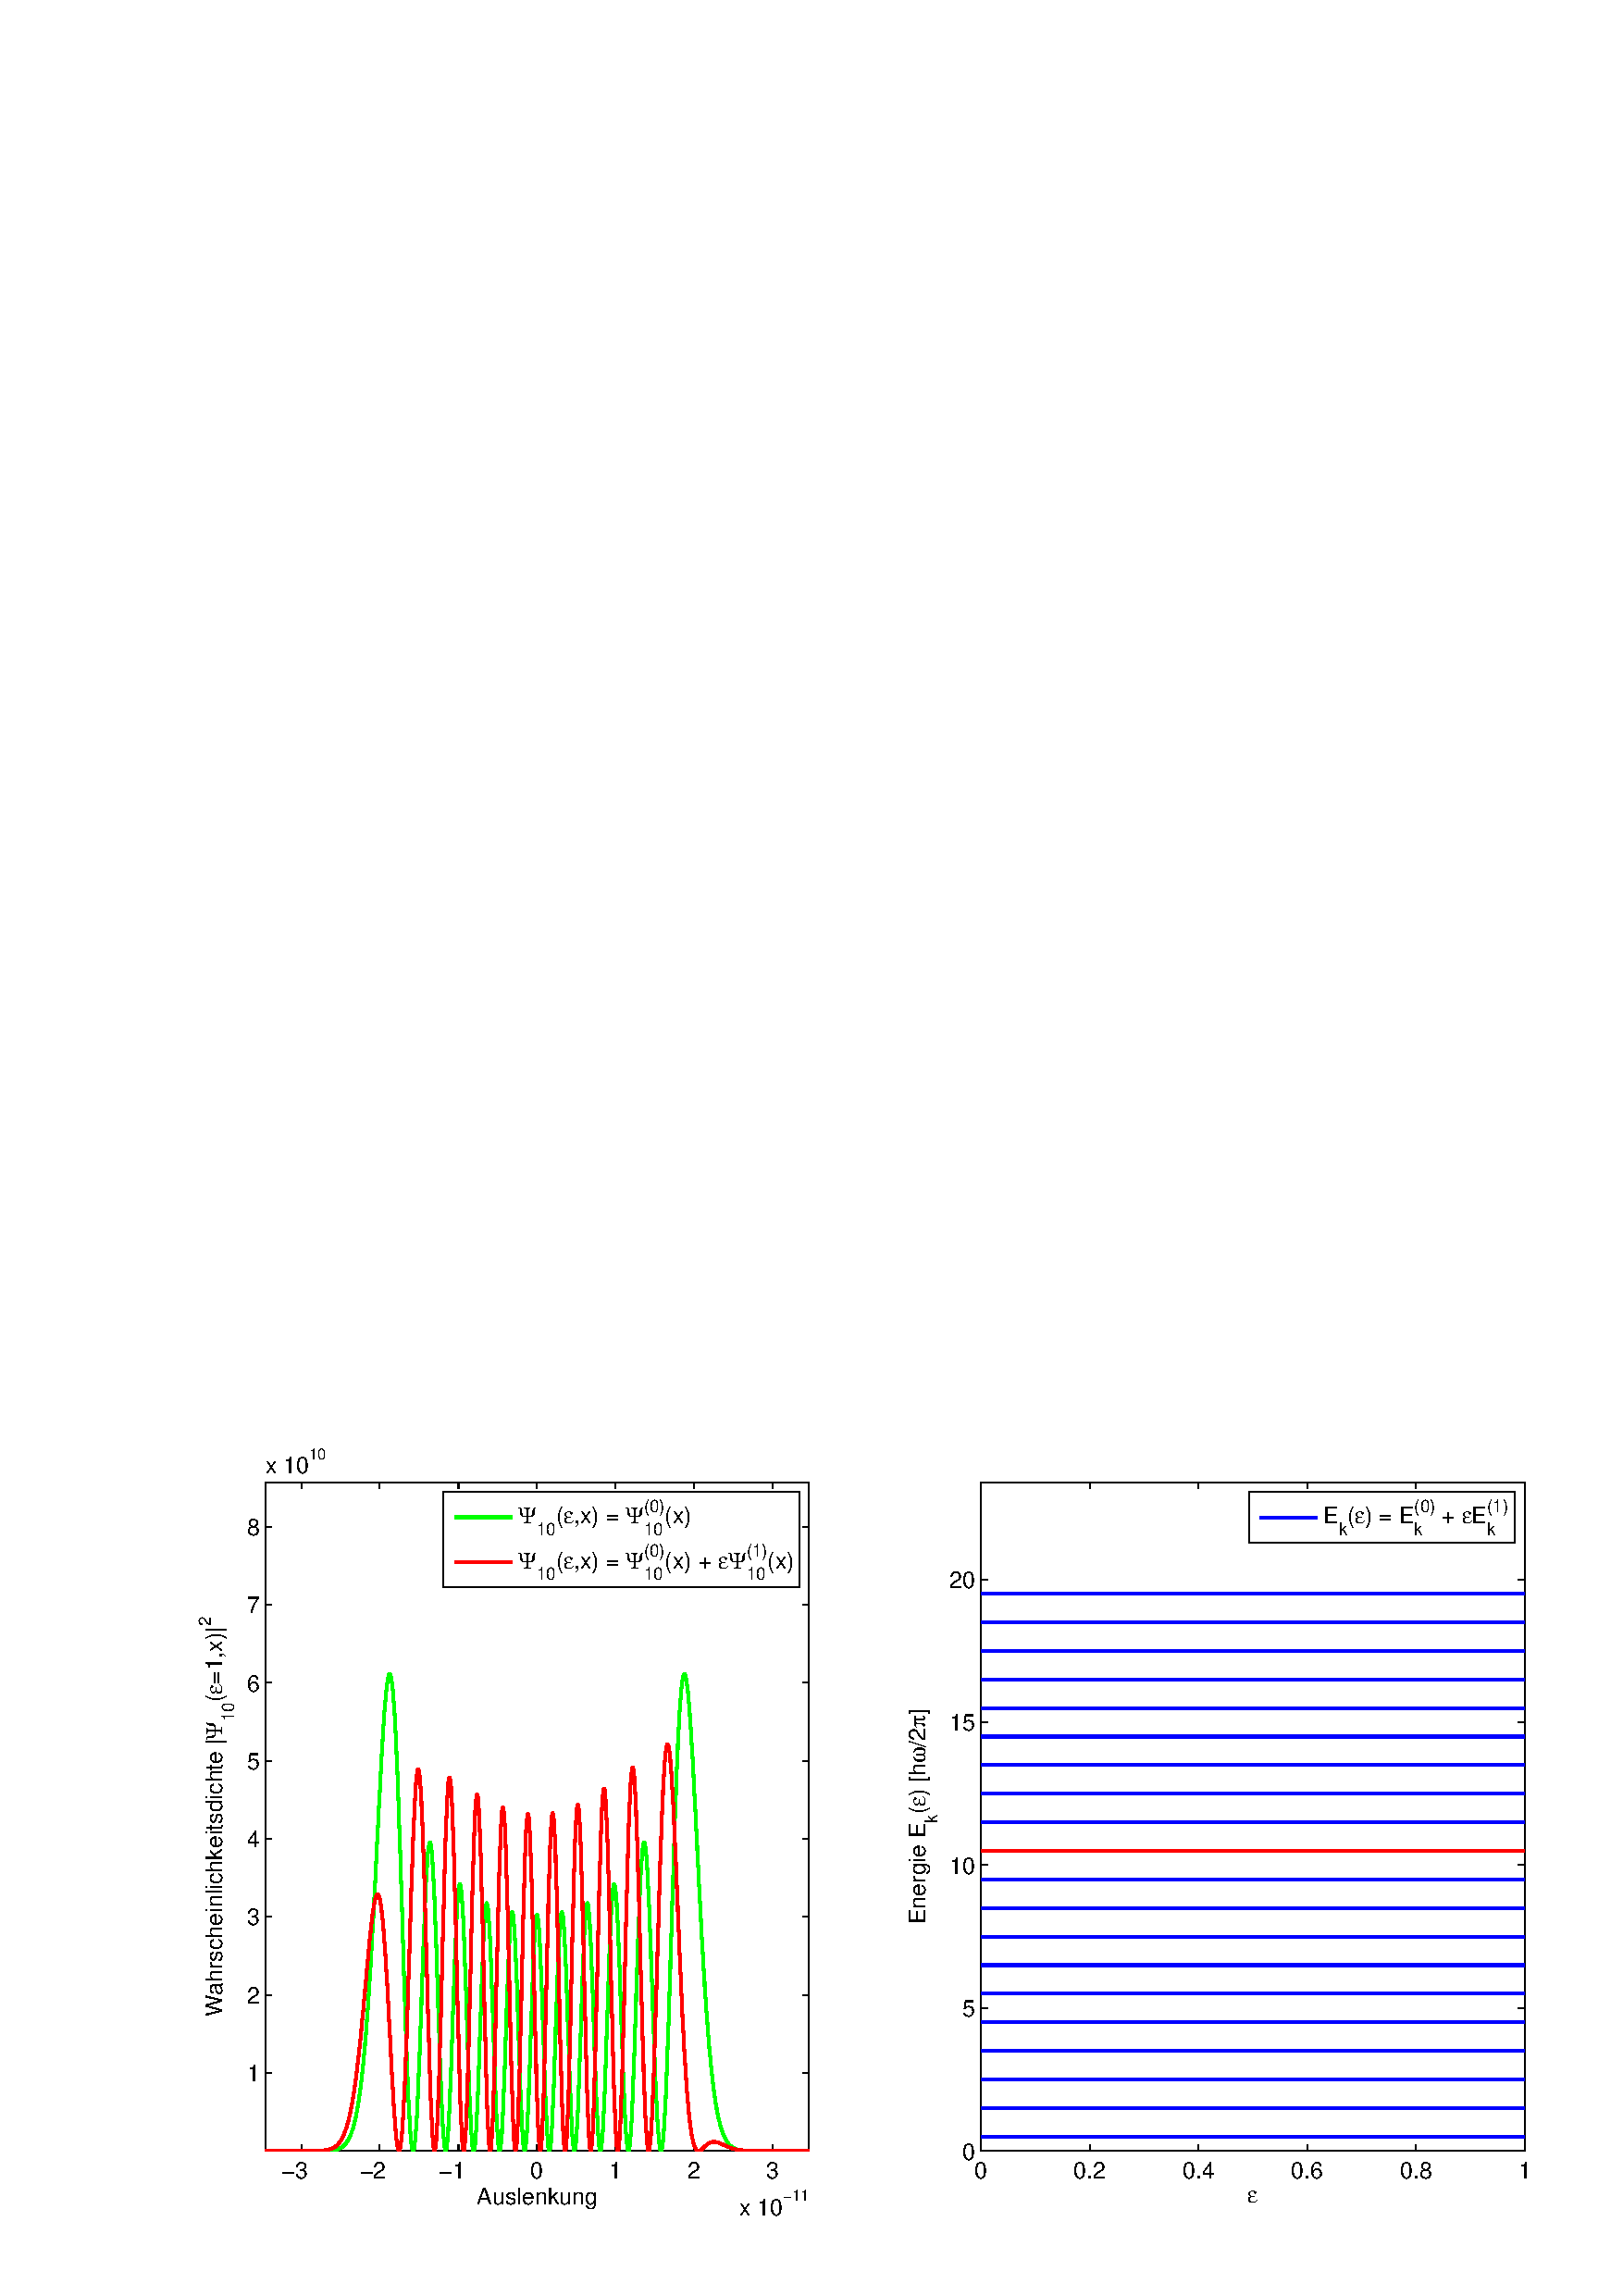
\includegraphics[width=0.8\textwidth]{anharmonisch/images/x3/Stoerung1Wellenfunktion.pdf}
\caption{10. Wellenfunktion und Energieniveaus in erster N"aherung
\label{skript:x3_Stoerung1Wellenfunktion}}
\end{figure}

Auf der Abbildung~\ref{skript:x3_Stoerung1Wellenfunktion} sieht man die 10. Wellenfunktion und die Energieniveaus in erster N"aherung. Man kann gut erkennen, dass sich die Energieniveaus nicht verschoben haben.

\begin{figure}[h]	%Bild Stoerung1Skalare.pdf
\centering
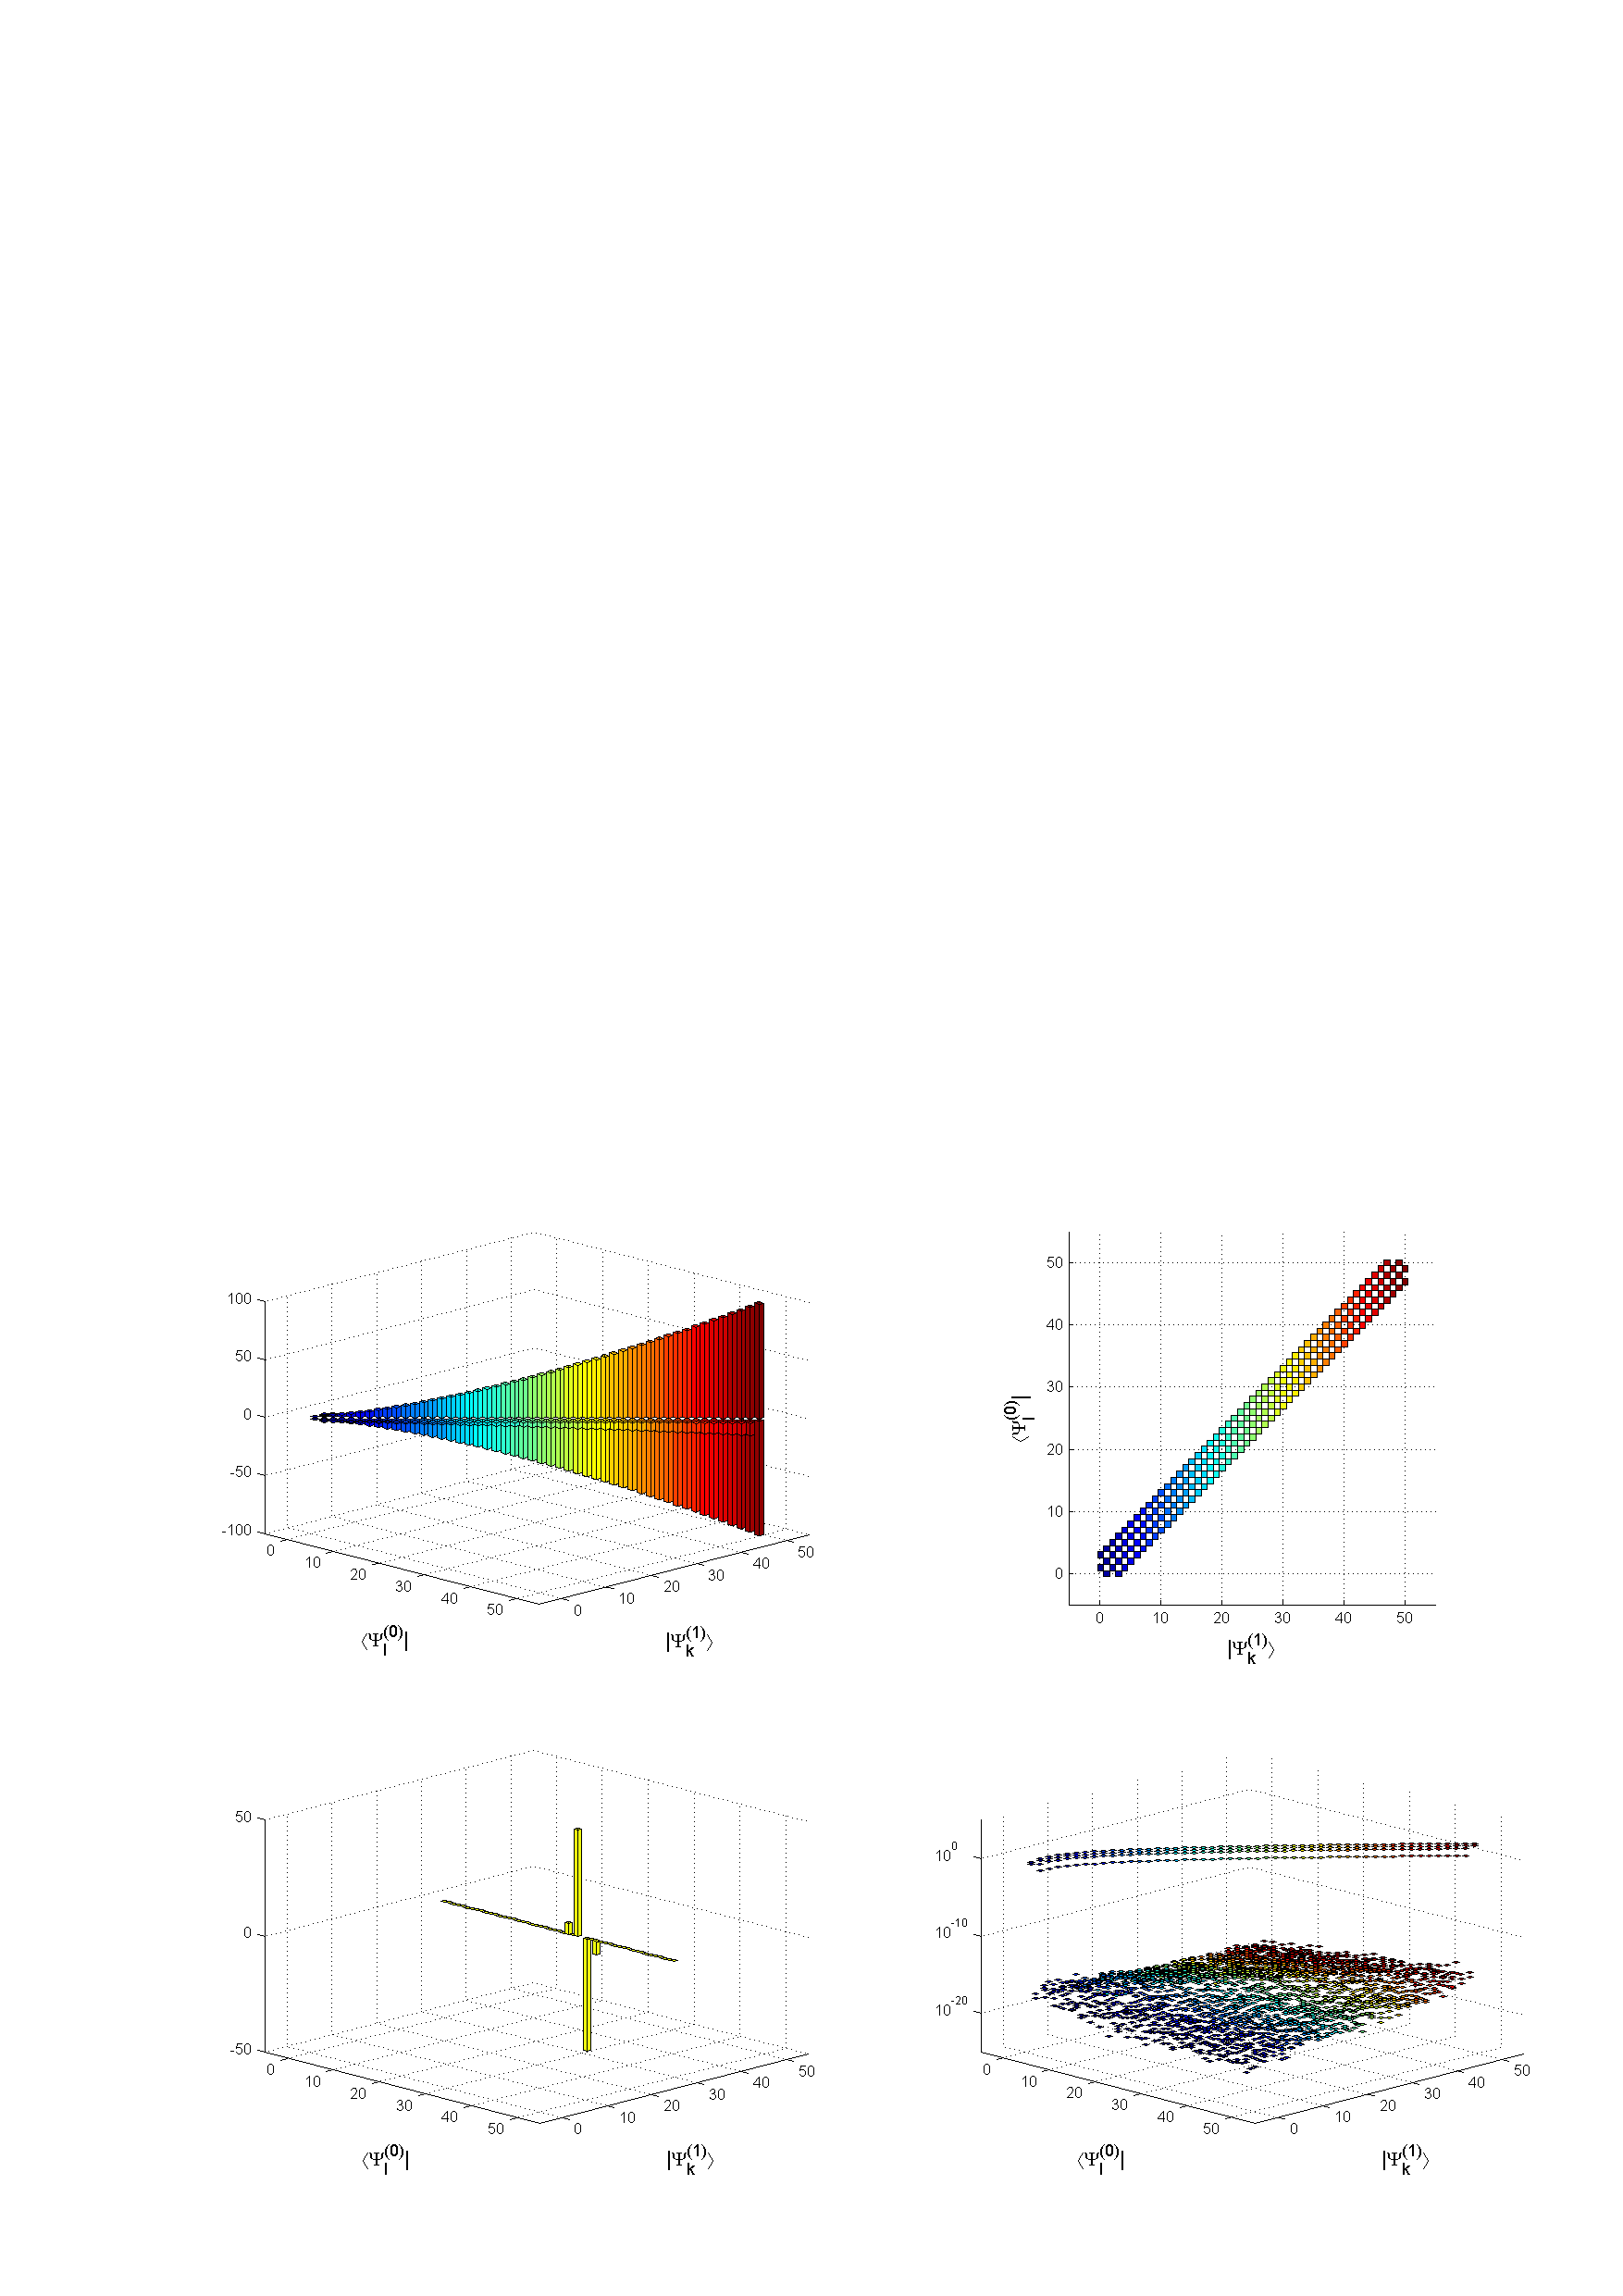
\includegraphics[width=1.0\textwidth]{anharmonisch/images/x3/Stoerung1Skalare.pdf}
\caption{Skalarprodukte $\langle\Psi_l^{(0)}|\Psi_k^{(1)}\rangle$ in erster N"aherung
\label{skript:x3_Stoerung1Skalare}}
\end{figure}

Auf der Abbildung~\ref{skript:x3_Stoerung1Skalare} sieht man welche ungest"orten Wellenfunktionen $\Psi_l^{(0)}$ den gr"ossten Anteil an der gest"orten Wellenfunktion $\Psi_k^{(1)}$ in erster N"aherung haben. Das heisst, aus welchen bekannten Wellenfunktionen sich die neue Wellenfunktion zusammensetzt. In erster Näherung können diese Anteile positiv oder negativ sein. Der Fall $k=l$ wird auf diesen Abbildungen nicht dargestellt. Den gr"ossten Anteil ergibt sich durch die Wellenfunktionen, welche am n"achsten bei der urspr"unglichen Wellenfunktion sind. Dies war zu erwarten, da der Nenner von der Gleichung~\ref{skript:stoerungsloesung1ordnung} am kleinsten ist. Wellenfunktionen, bei welchen $l=k\pm 2,k\pm 4,\dots$ ist, geben keinen Anteil an die gest"orte Wellenfunktion, da sie orthogonal dazu stehen. Ausserdem kann man sehen, dass bei gr"osseren $k$ auch die Anteile anderen Wellenfuntionen $l\neq k$ linear gr"osser werden. In der logarithmischen darstellung sieht man das die Wellenfuntionen, welche weiter weg sind nur noch einen vernachl"assigbar kleinen Beitrag liefern. Grunds"atzlich ist aber auch dort eine Zuhnahme bei den gr"osseren Wellenfunktionen zu erkennen.


\begin{figure}[h]	%Bild EK2.pdf
\centering
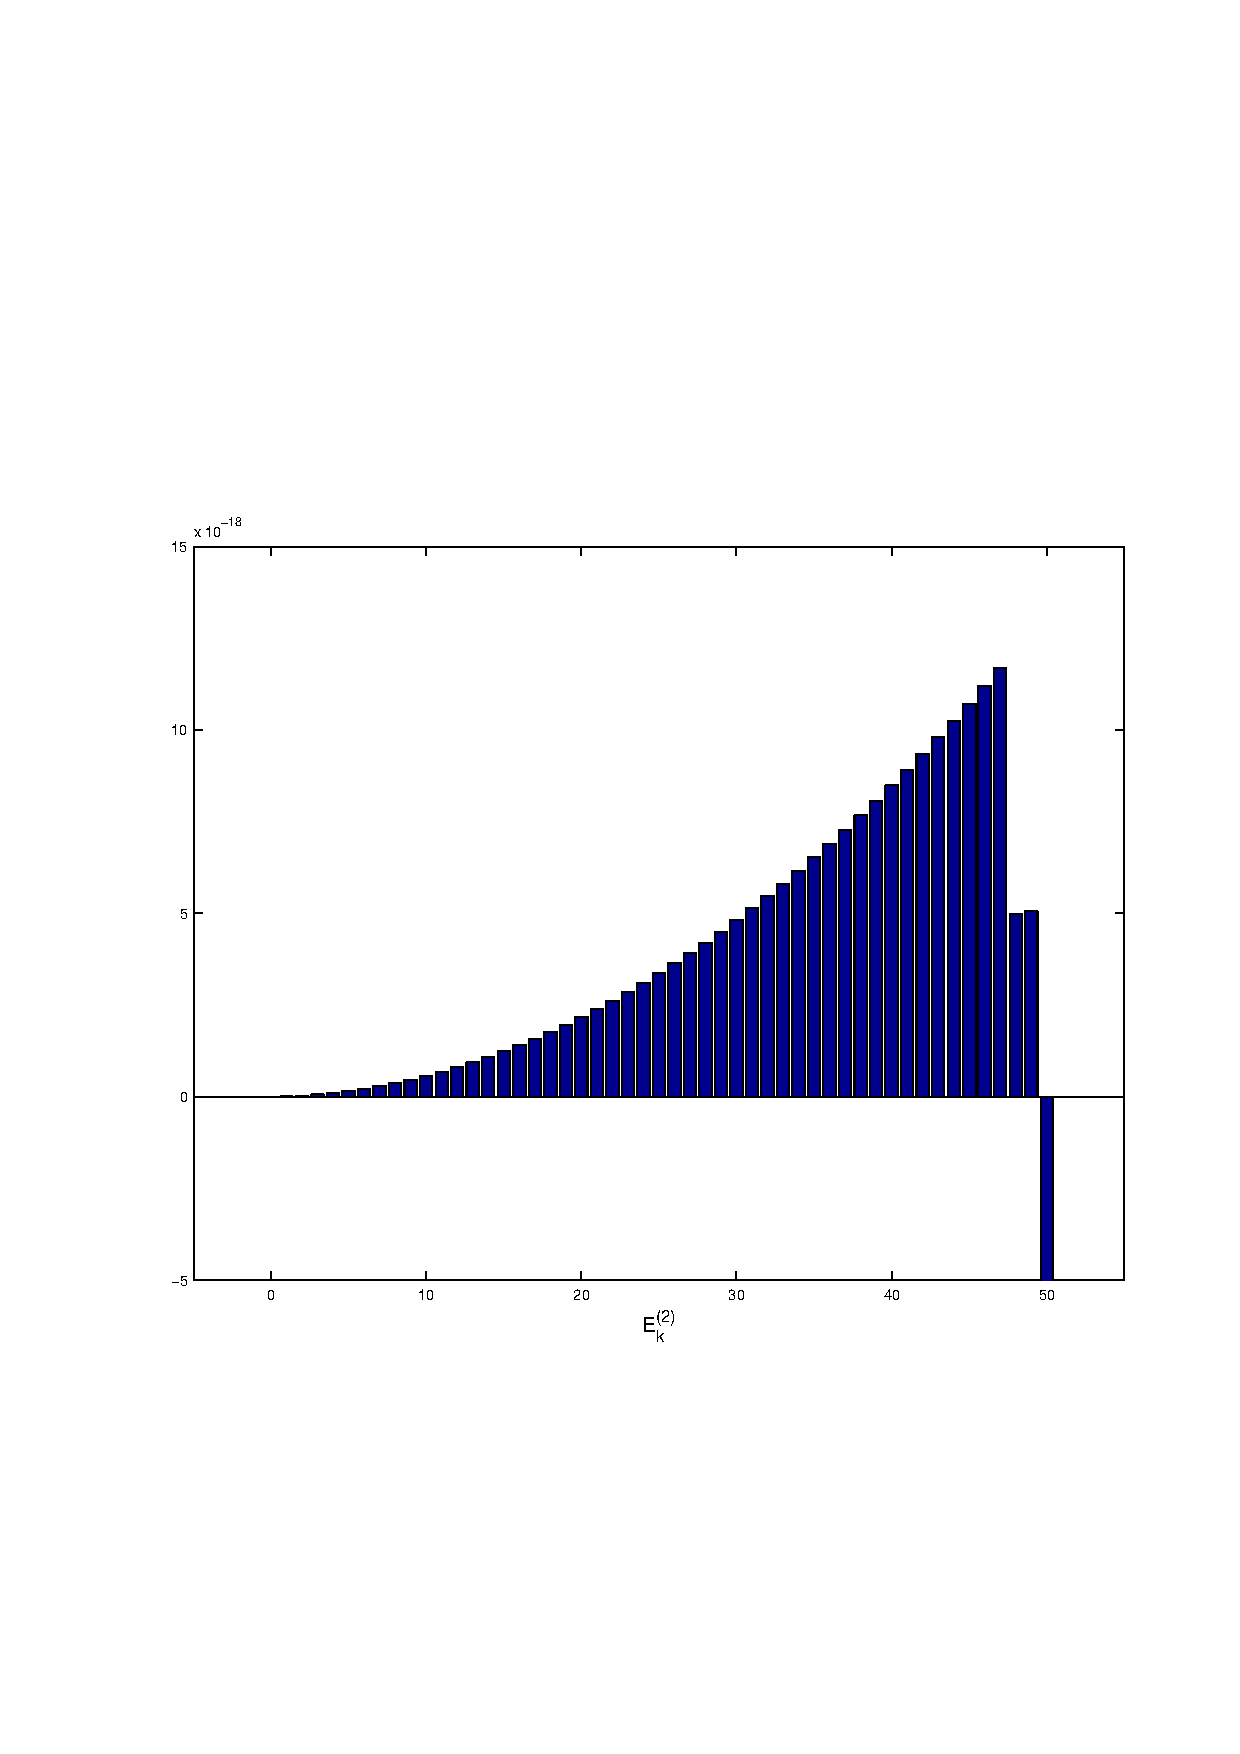
\includegraphics[width=0.6\textwidth]{anharmonisch/images/x3/EK2.pdf}
\caption{St"orung der Energieniveaus zweiter N"aherung
\label{skript:x3_EK2}}
\end{figure}

Auf der Abbildung~\ref{skript:x3_EK2} sieht man die "Anderung der Energieniveaus in zweiter N"aherung. Man kann klar Erkennen, dass die Abweichungen zum harmonischen Fall, bei h"oheren Energieniveaus immer gr"osser wird. Die Unstetigkeit bei den letzten drei Energieniveaus ist darauf zur"uckzuf"uhren, dass f"ur die Berechnung dieser Terme, Daten von noch h"oheren Energieniveaus ben"otig werden, welche nicht mehr berechnet wurden.

\begin{figure}[h]	%Bild Stoerung2Wellenfunktion.pdf
\centering
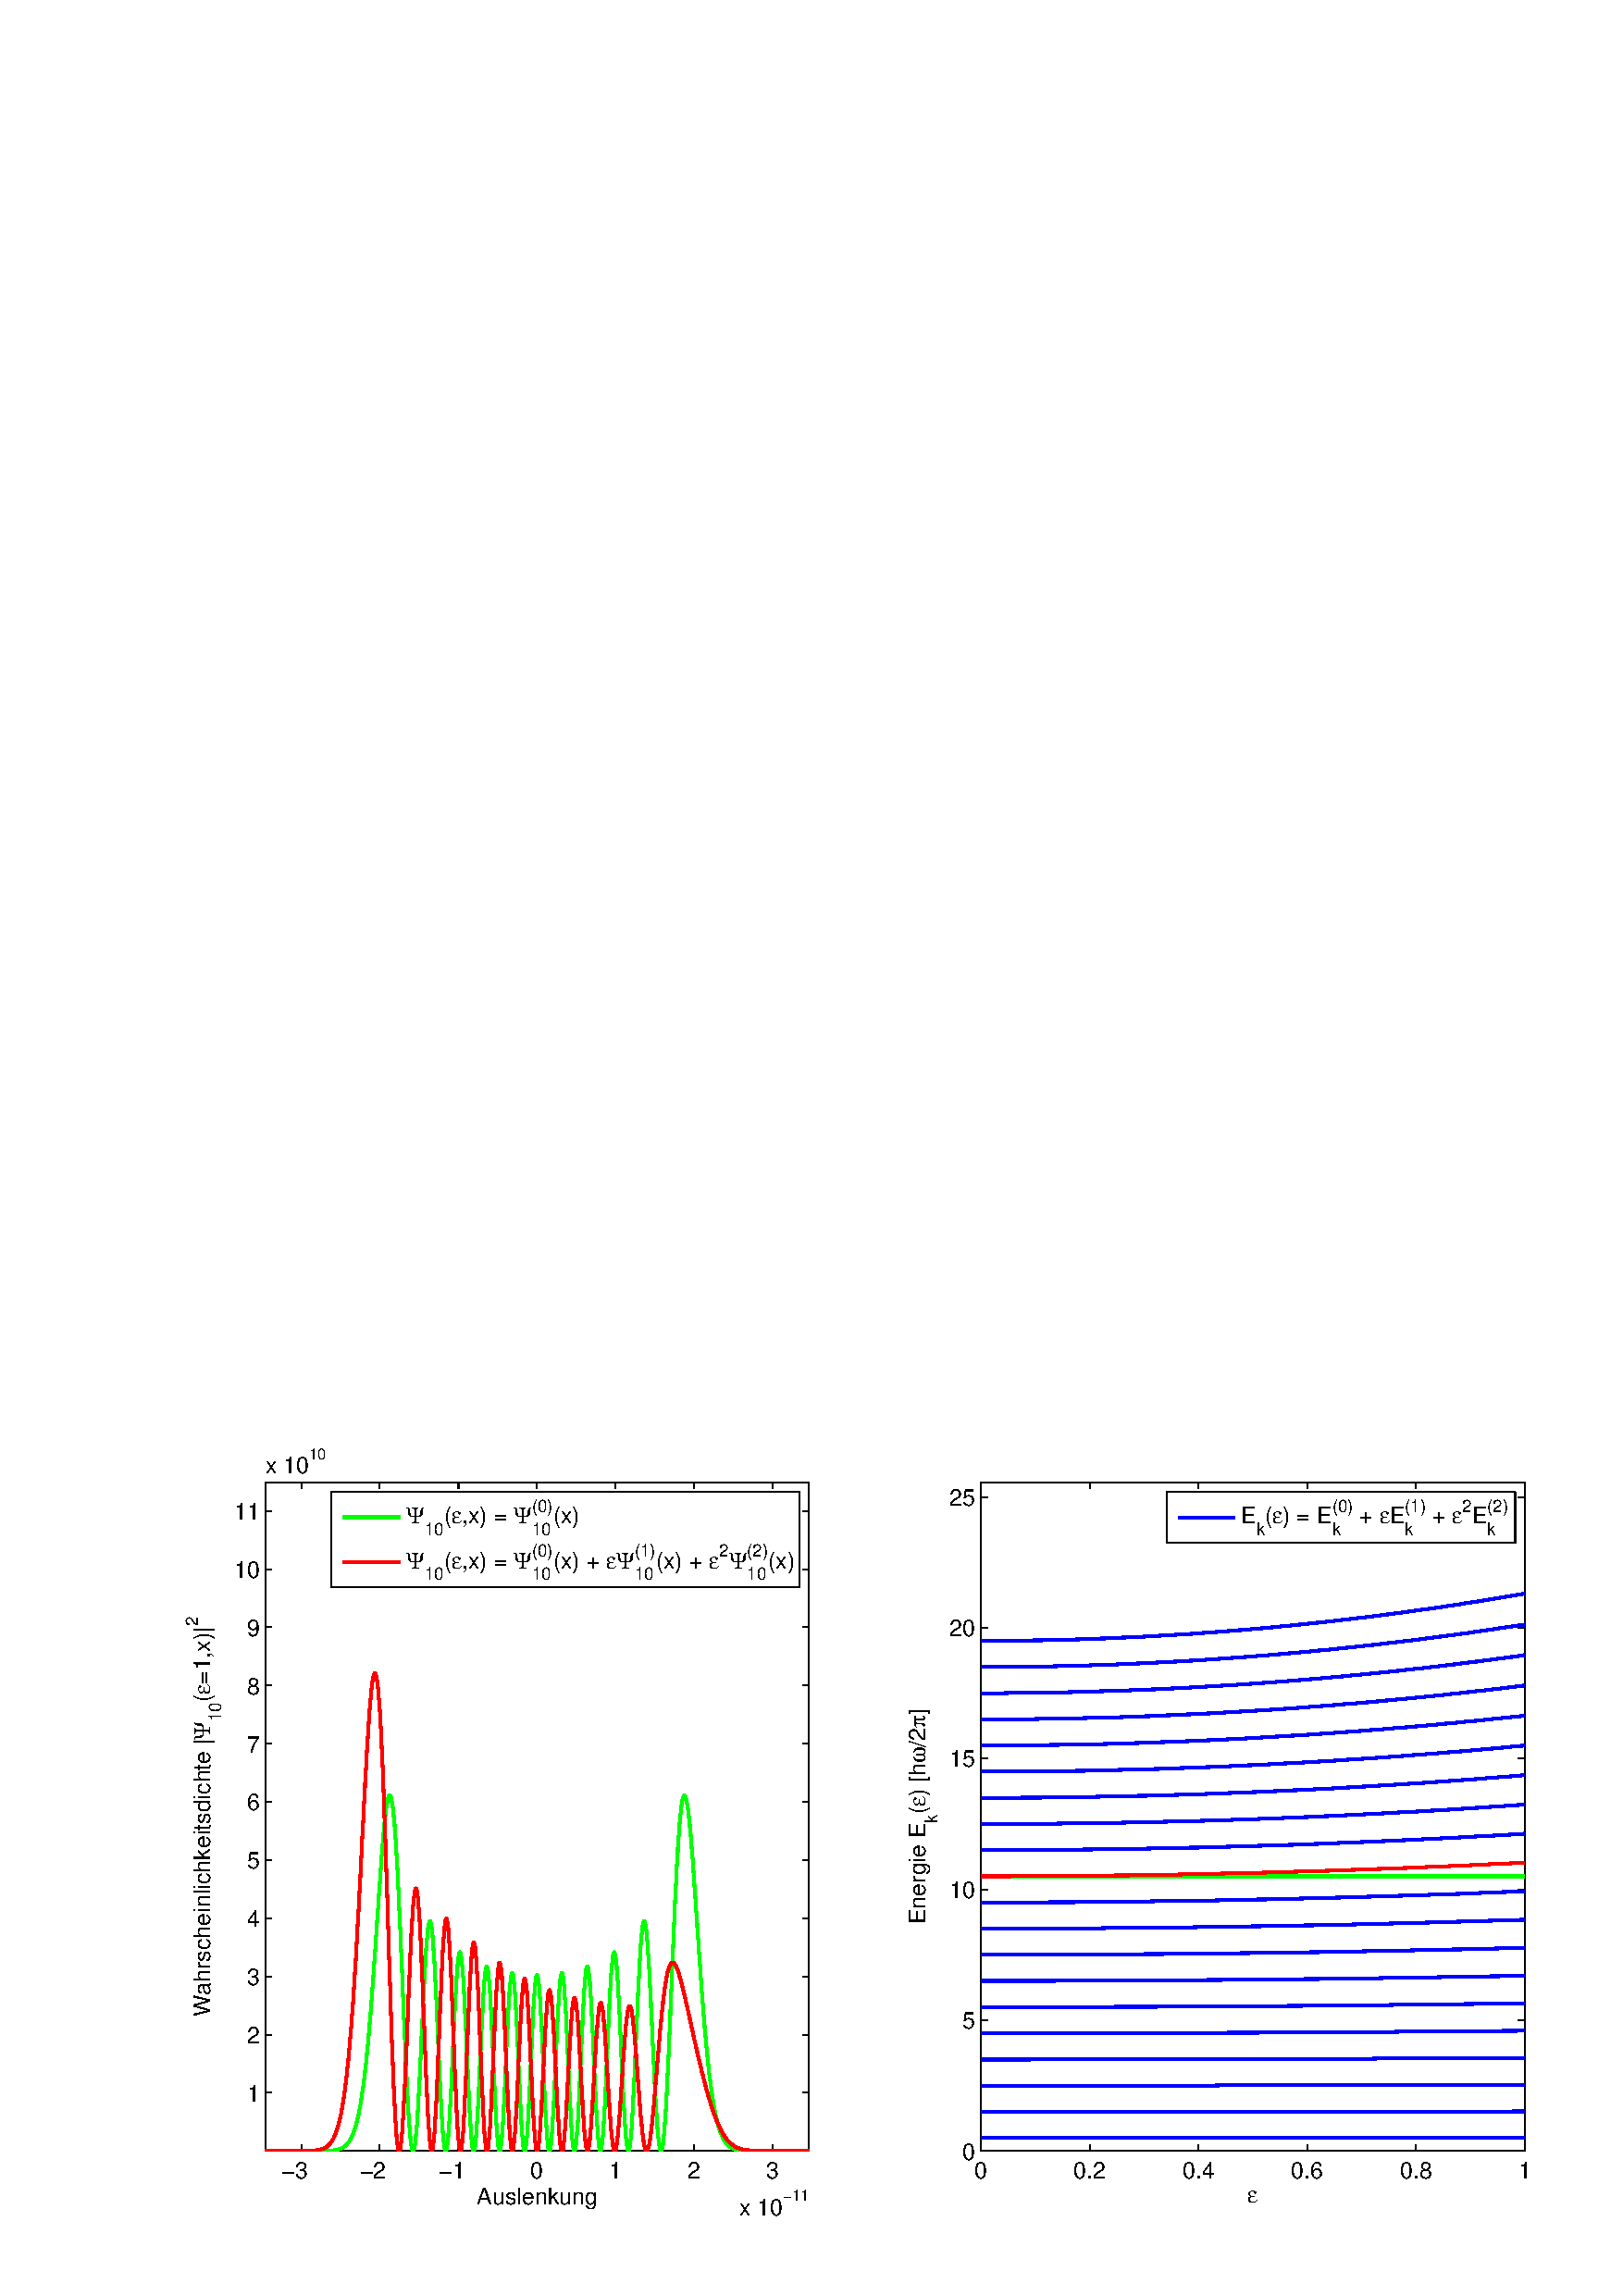
\includegraphics[width=0.8\textwidth]{anharmonisch/images/x3/Stoerung2Wellenfunktion.pdf}
\caption{10. Wellenfunktion und Energieniveaus in zweiter N"aherung
\label{skript:x3_Stoerung1Wellenfunktion}}
\end{figure}

Auf der Abbildung~\ref{skript:x3_Stoerung1Wellenfunktion} sieht man die 10. Wellenfunktion und die Energieniveaus in zweiter N"aherung. Die Aufenthaltswarscheinlichkeit hat sich nach links verschoben. Bei den h"oheren Energieniveaus sieht man, dass es nicht mehr nur linear ansteigt sondern auch der quadratische Term zum Tragen kommt.

\begin{figure}[h]	%Bild Stoerung2Skalare.pdf
\centering
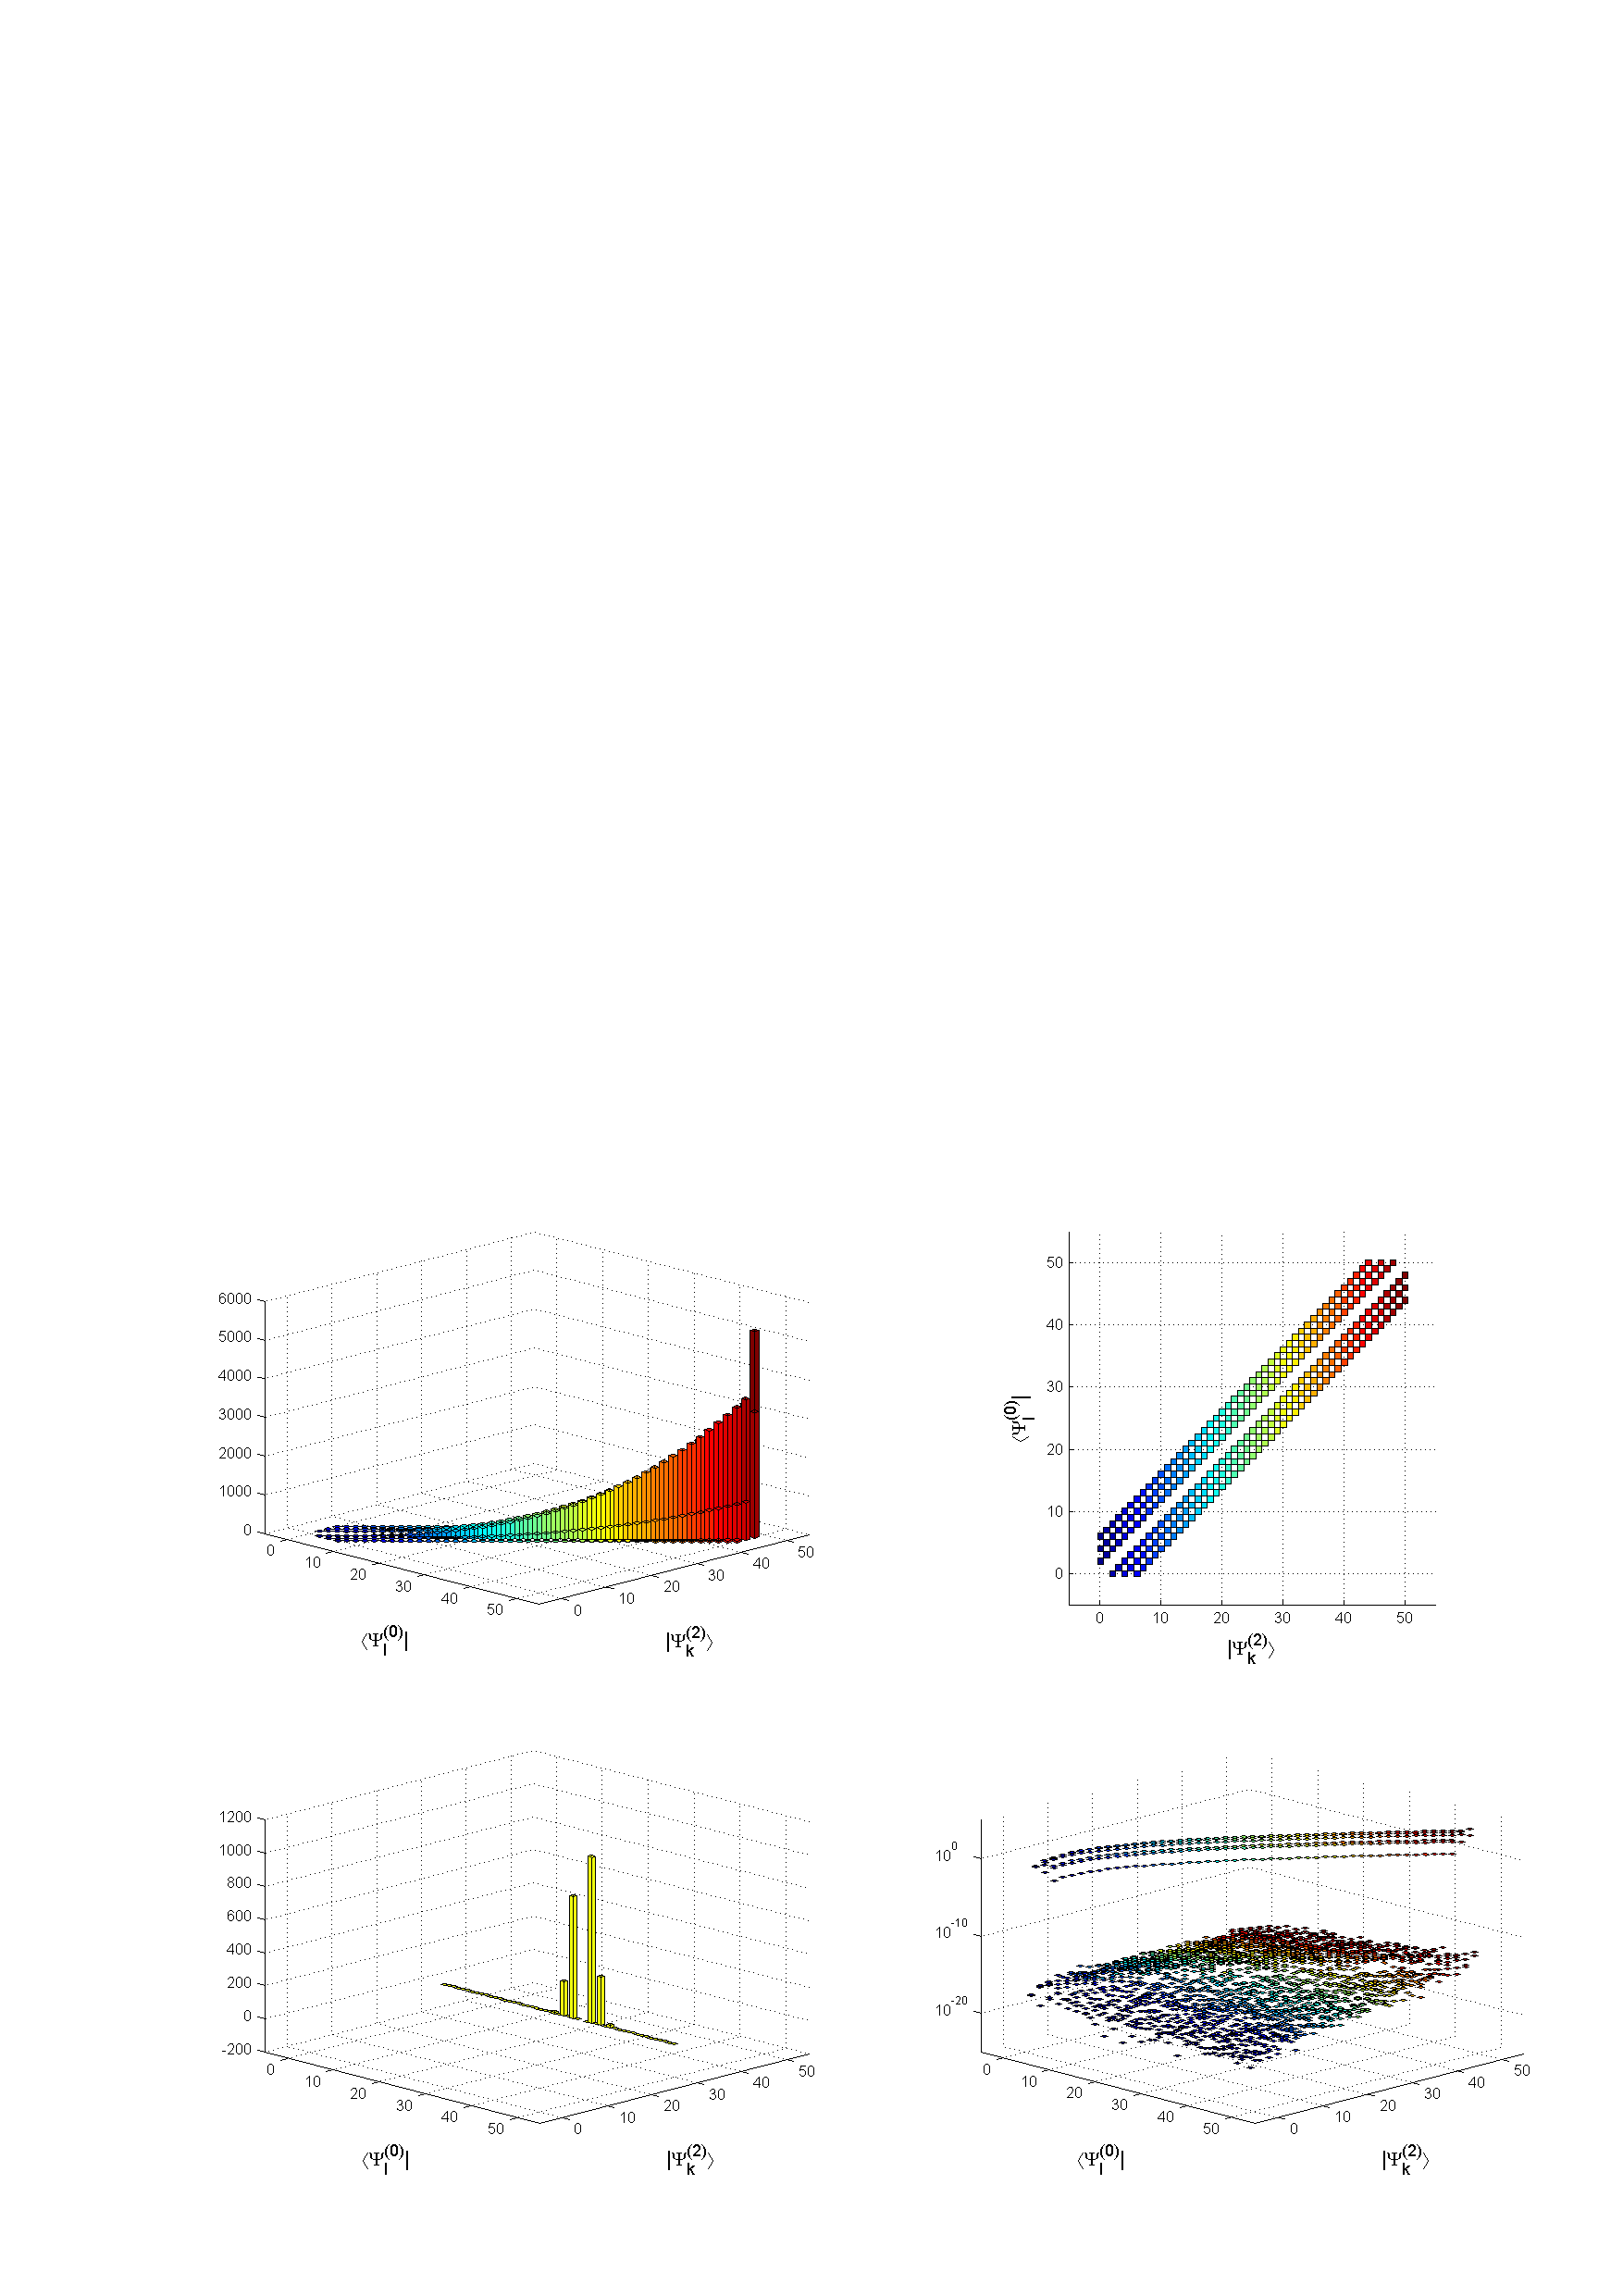
\includegraphics[width=1.0\textwidth]{anharmonisch/images/x3/Stoerung2Skalare.pdf}
\caption{Skalarprodukte $\langle\Psi_l^{(0)}|\Psi_k^{(2)}\rangle$ in zweiter N"aherung
\label{skript:x3_Stoerung2Skalare}}
\end{figure}

Auf der Abbildung~\ref{skript:x3_Stoerung1Skalare} sieht man welche ungest"orten Wellenfunktionen $\Psi_l^{(0)}$ den gr"ossten Anteil an der gest"orten Wellenfunktion $\Psi_k^{(2)}$ in zweiter N"aherung haben. In zweiter Näherung sind diese Anteile immer positiv. Der Fall $k=l$ wird auf diesen Abbildungen nicht dargestellt.  Wellenfunktionen, bei welchen $l=k\pm 1,k\pm 3,\dots$ ist, geben keinen Anteil an die gest"orte Wellenfunktion, da sie orthogonal dazu stehen. Ausserdem kann man sehen, dass bei gr"osseren $k$ auch die Anteile anderen Wellenfuntionen $l\neq k$ quadratisch gr"osser werden. In der logarithmischen darstellung sieht man das die Wellenfuntionen, welche weiter weg sind nur noch einen vernachl"assigbar kleinen Beitrag liefern. Grunds"atzlich ist aber auch dort eine Zuhnahme bei den gr"osseren Wellenfunktionen zu erkennen.

			%Zweites Beispiel
\subsection{Zweites Beispiel $bQ^4$}

\begin{figure}[h]	%Bild EK1.pdf
\centering
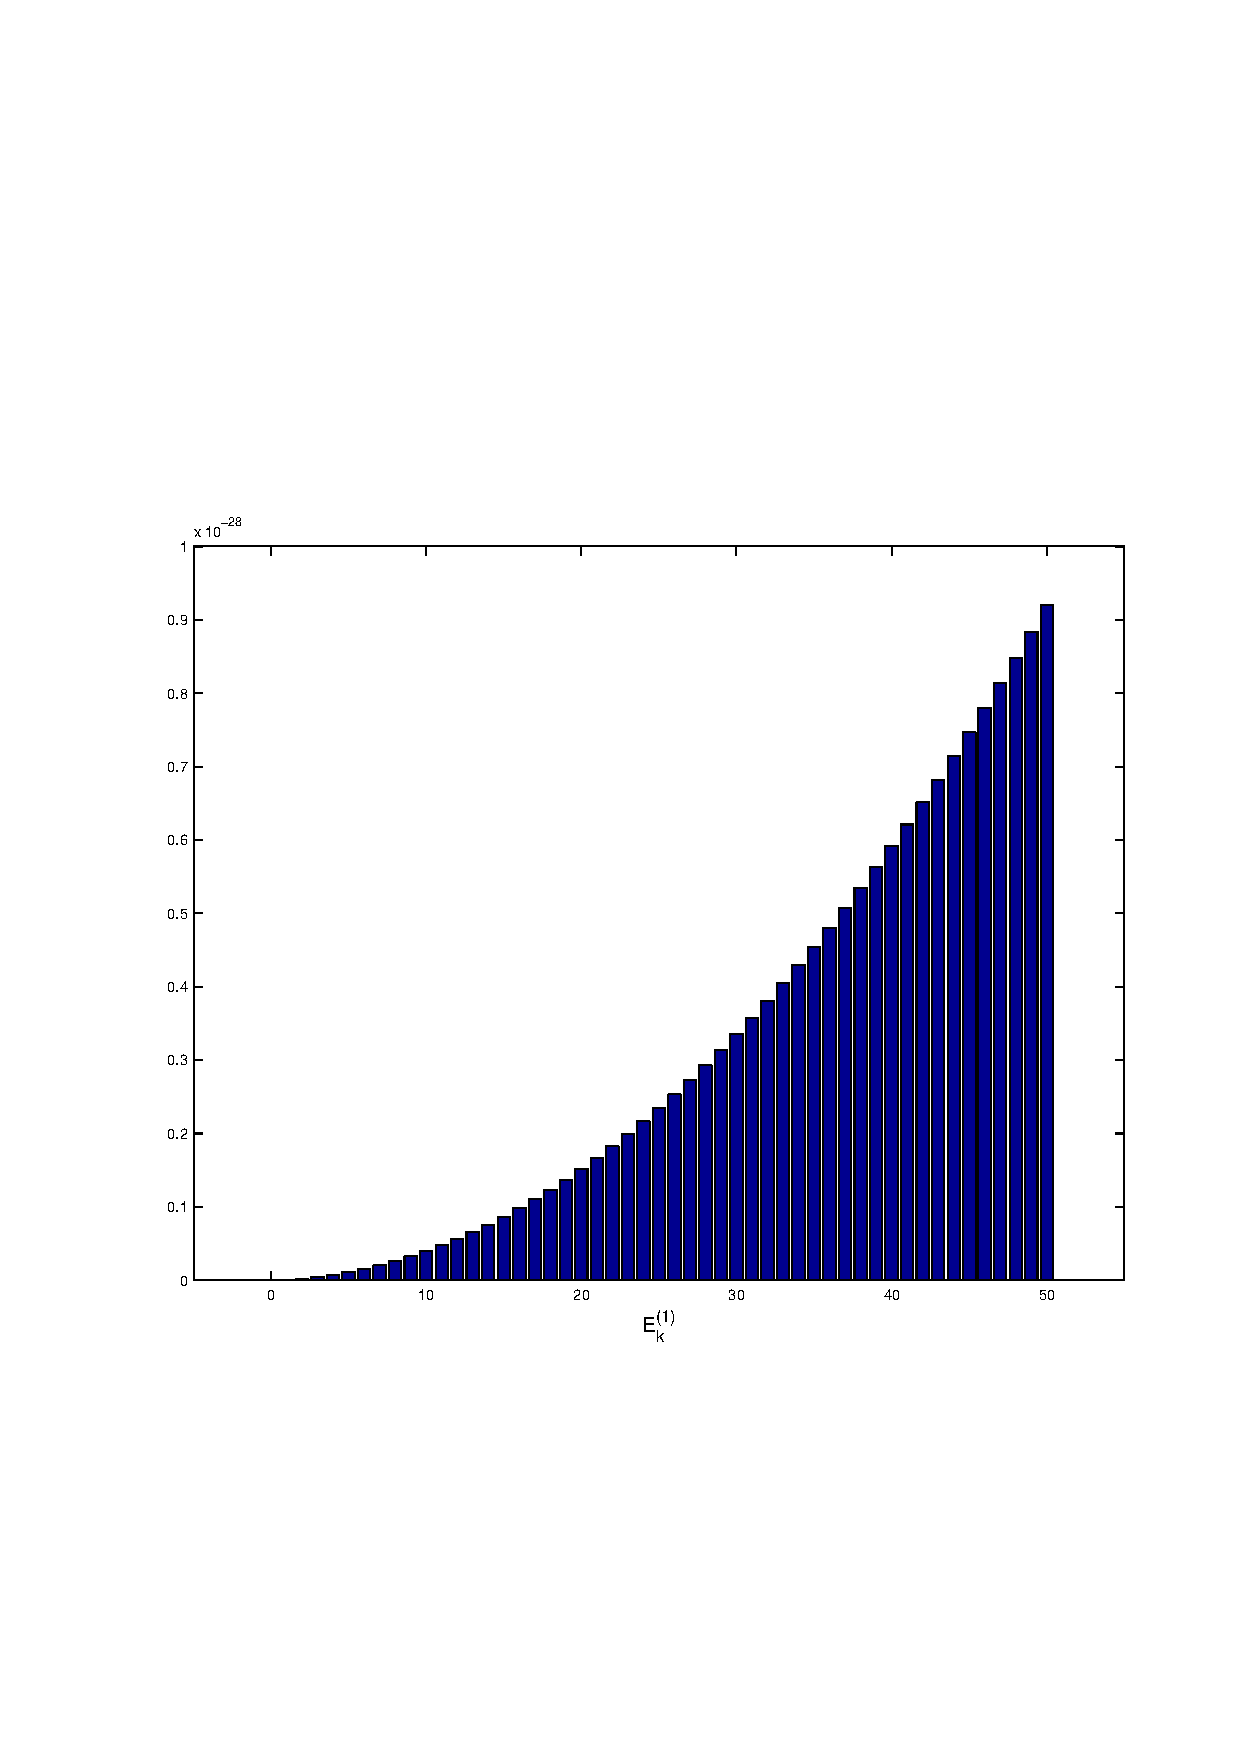
\includegraphics[width=0.6\textwidth]{anharmonisch/images/x4/EK1.pdf}
\caption{St"orung der Energieniveaus erster N"aherung
\label{skript:x4_EK1}}
\end{figure}

Auf der Abbildung~\ref{skript:x4_EK1} sieht man die "Anderung der Energieniveaus in erster N"aherung. 

\begin{figure}[h]	%Bild Stoerung1Wellenfunktion.pdf
\centering
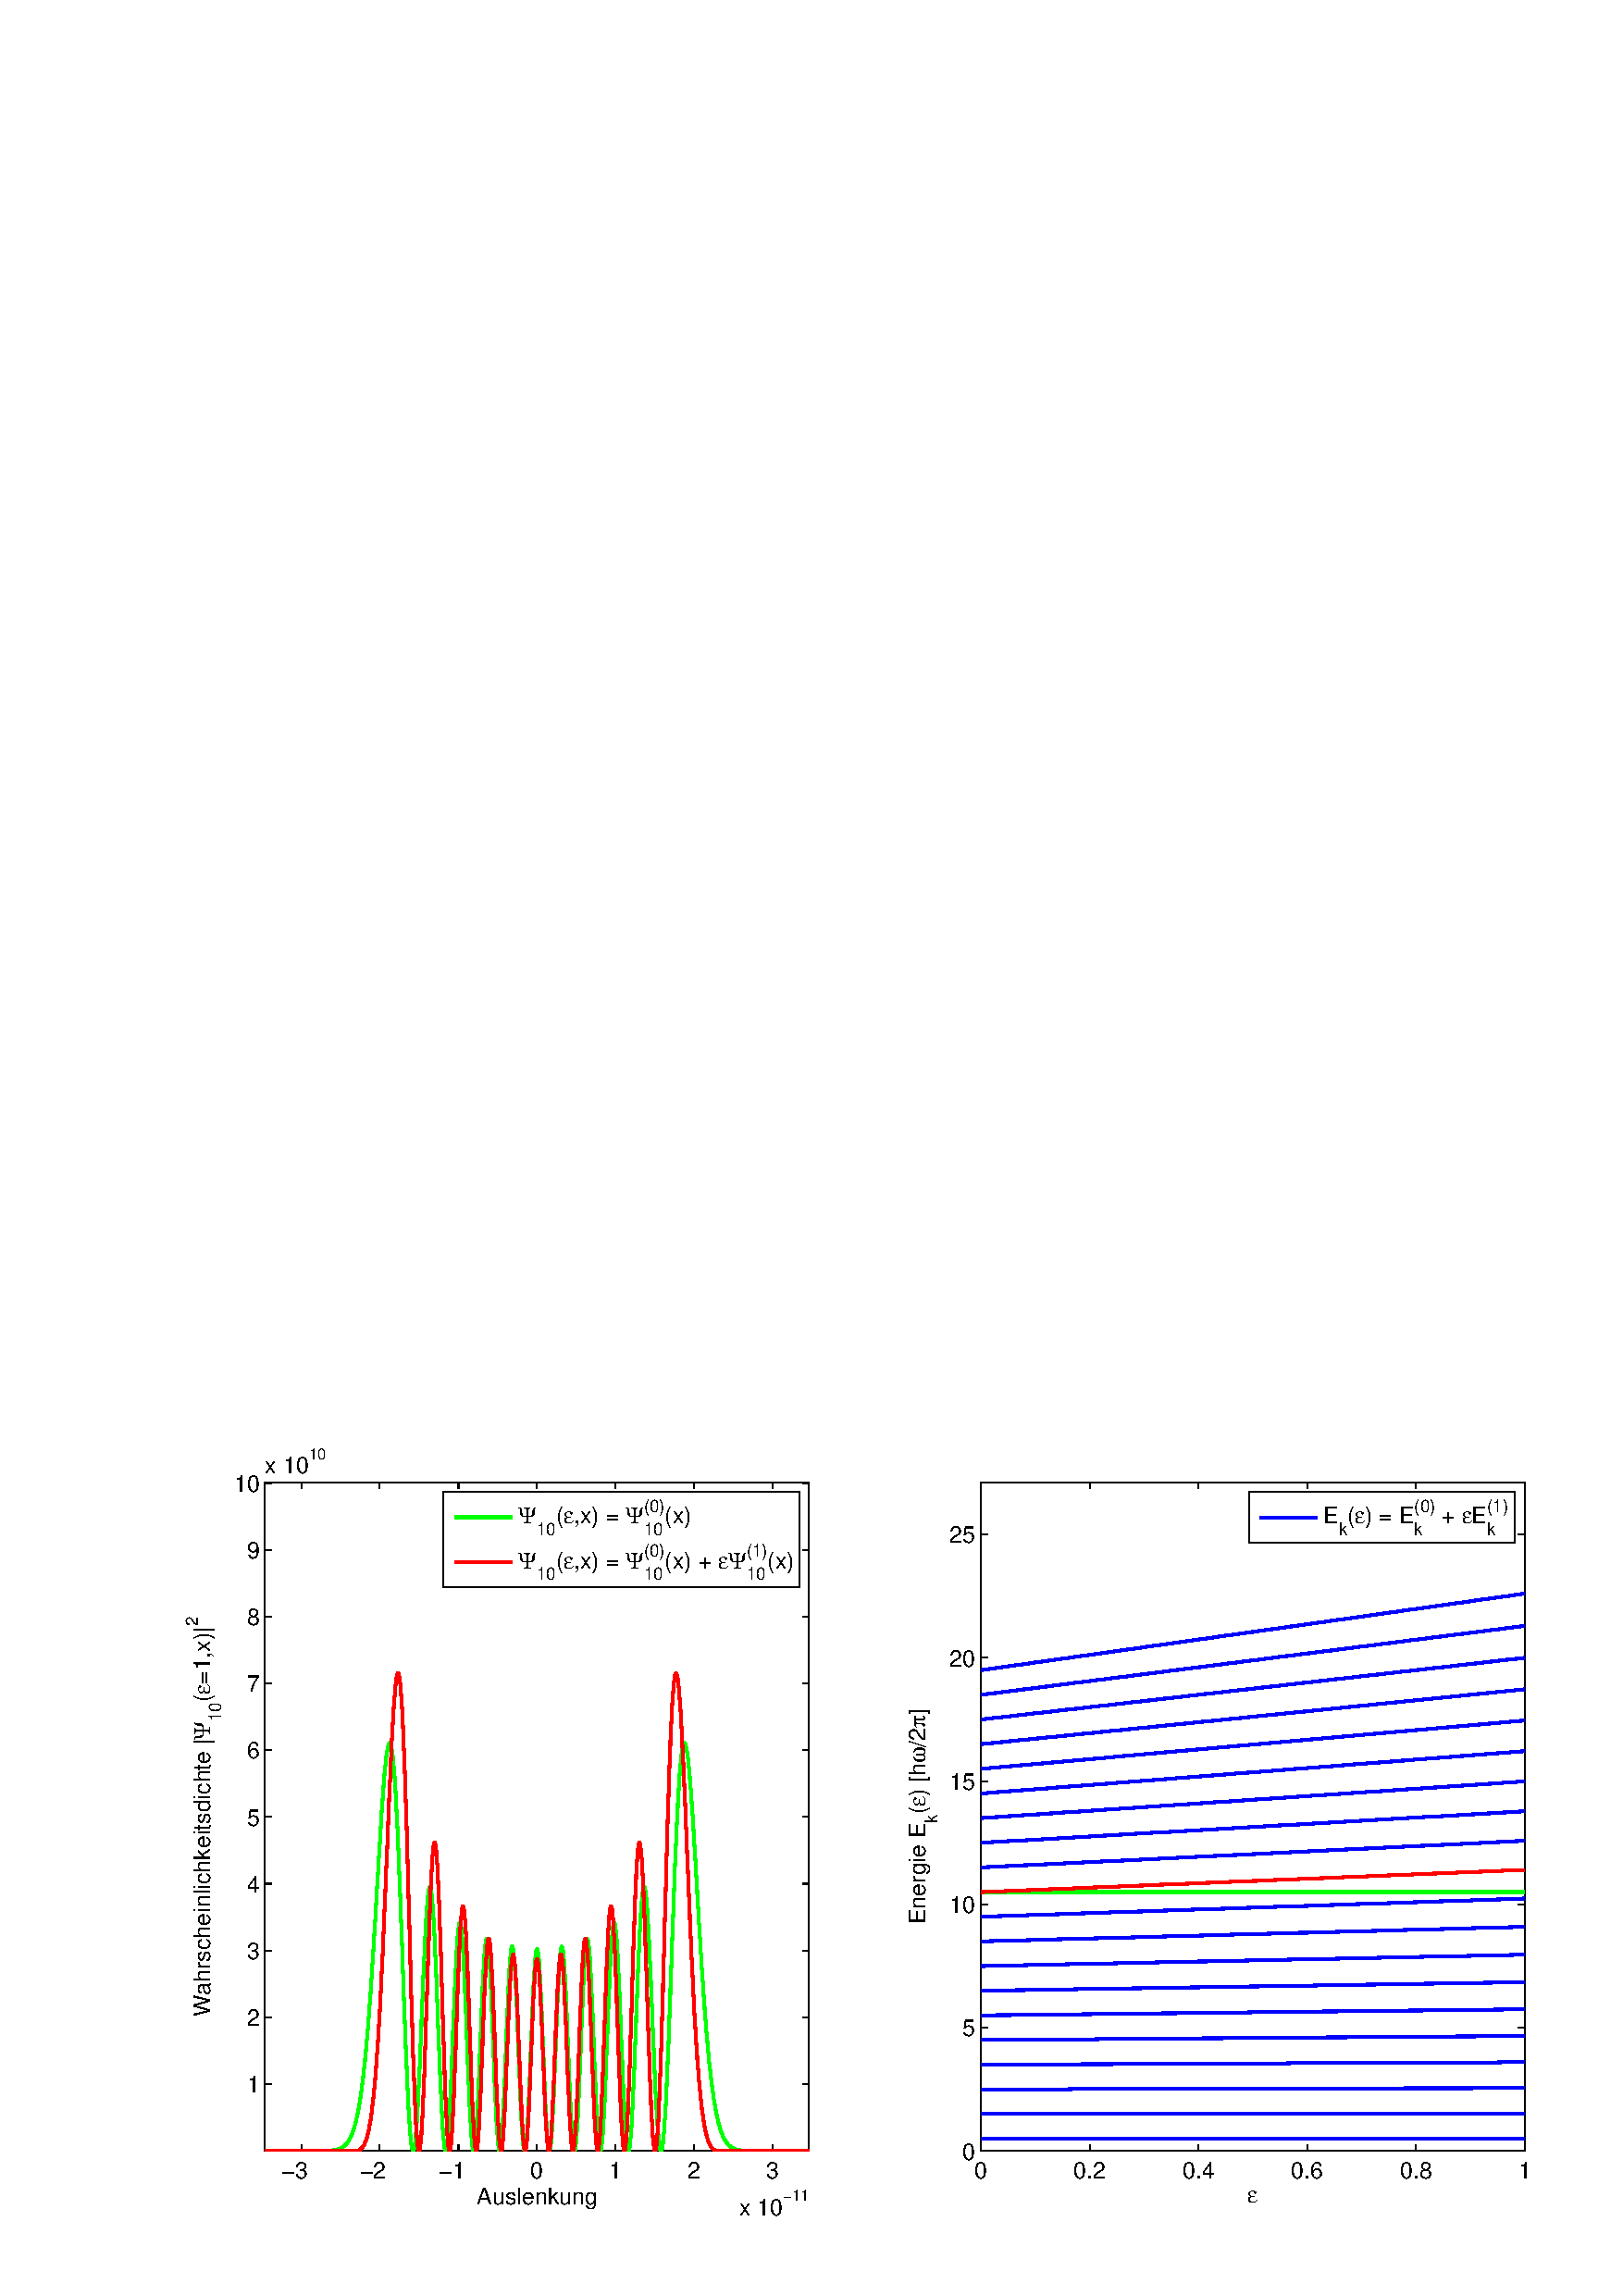
\includegraphics[width=0.8\textwidth]{anharmonisch/images/x4/Stoerung1Wellenfunktion.pdf}
\caption{10. Wellenfunktion und Energieniveaus in erster N"aherung
\label{skript:x4_Stoerung1Wellenfunktion}}
\end{figure}

Auf der Abbildung~\ref{skript:x4_Stoerung1Wellenfunktion} sieht man die 10. Wellenfunktion und die Energieniveaus in erster N"aherung. Die Aufenthaltswahrscheinlichkeit wird ein wenig zusammengedrückt und ist aussen noch deutlich höher als in der mitte. Die Energieniveaus verschieben sich bei gr"osseren $\varepsilon$ nach oben. Bei tiefen Energieniveaus ist die Verschibung noch sehr gering. Je h"oheren Energieniveau, desto gr"osser ist die Verschiebung.

\begin{figure}[h]	%Bild Stoerung1Skalare.pdf
\centering
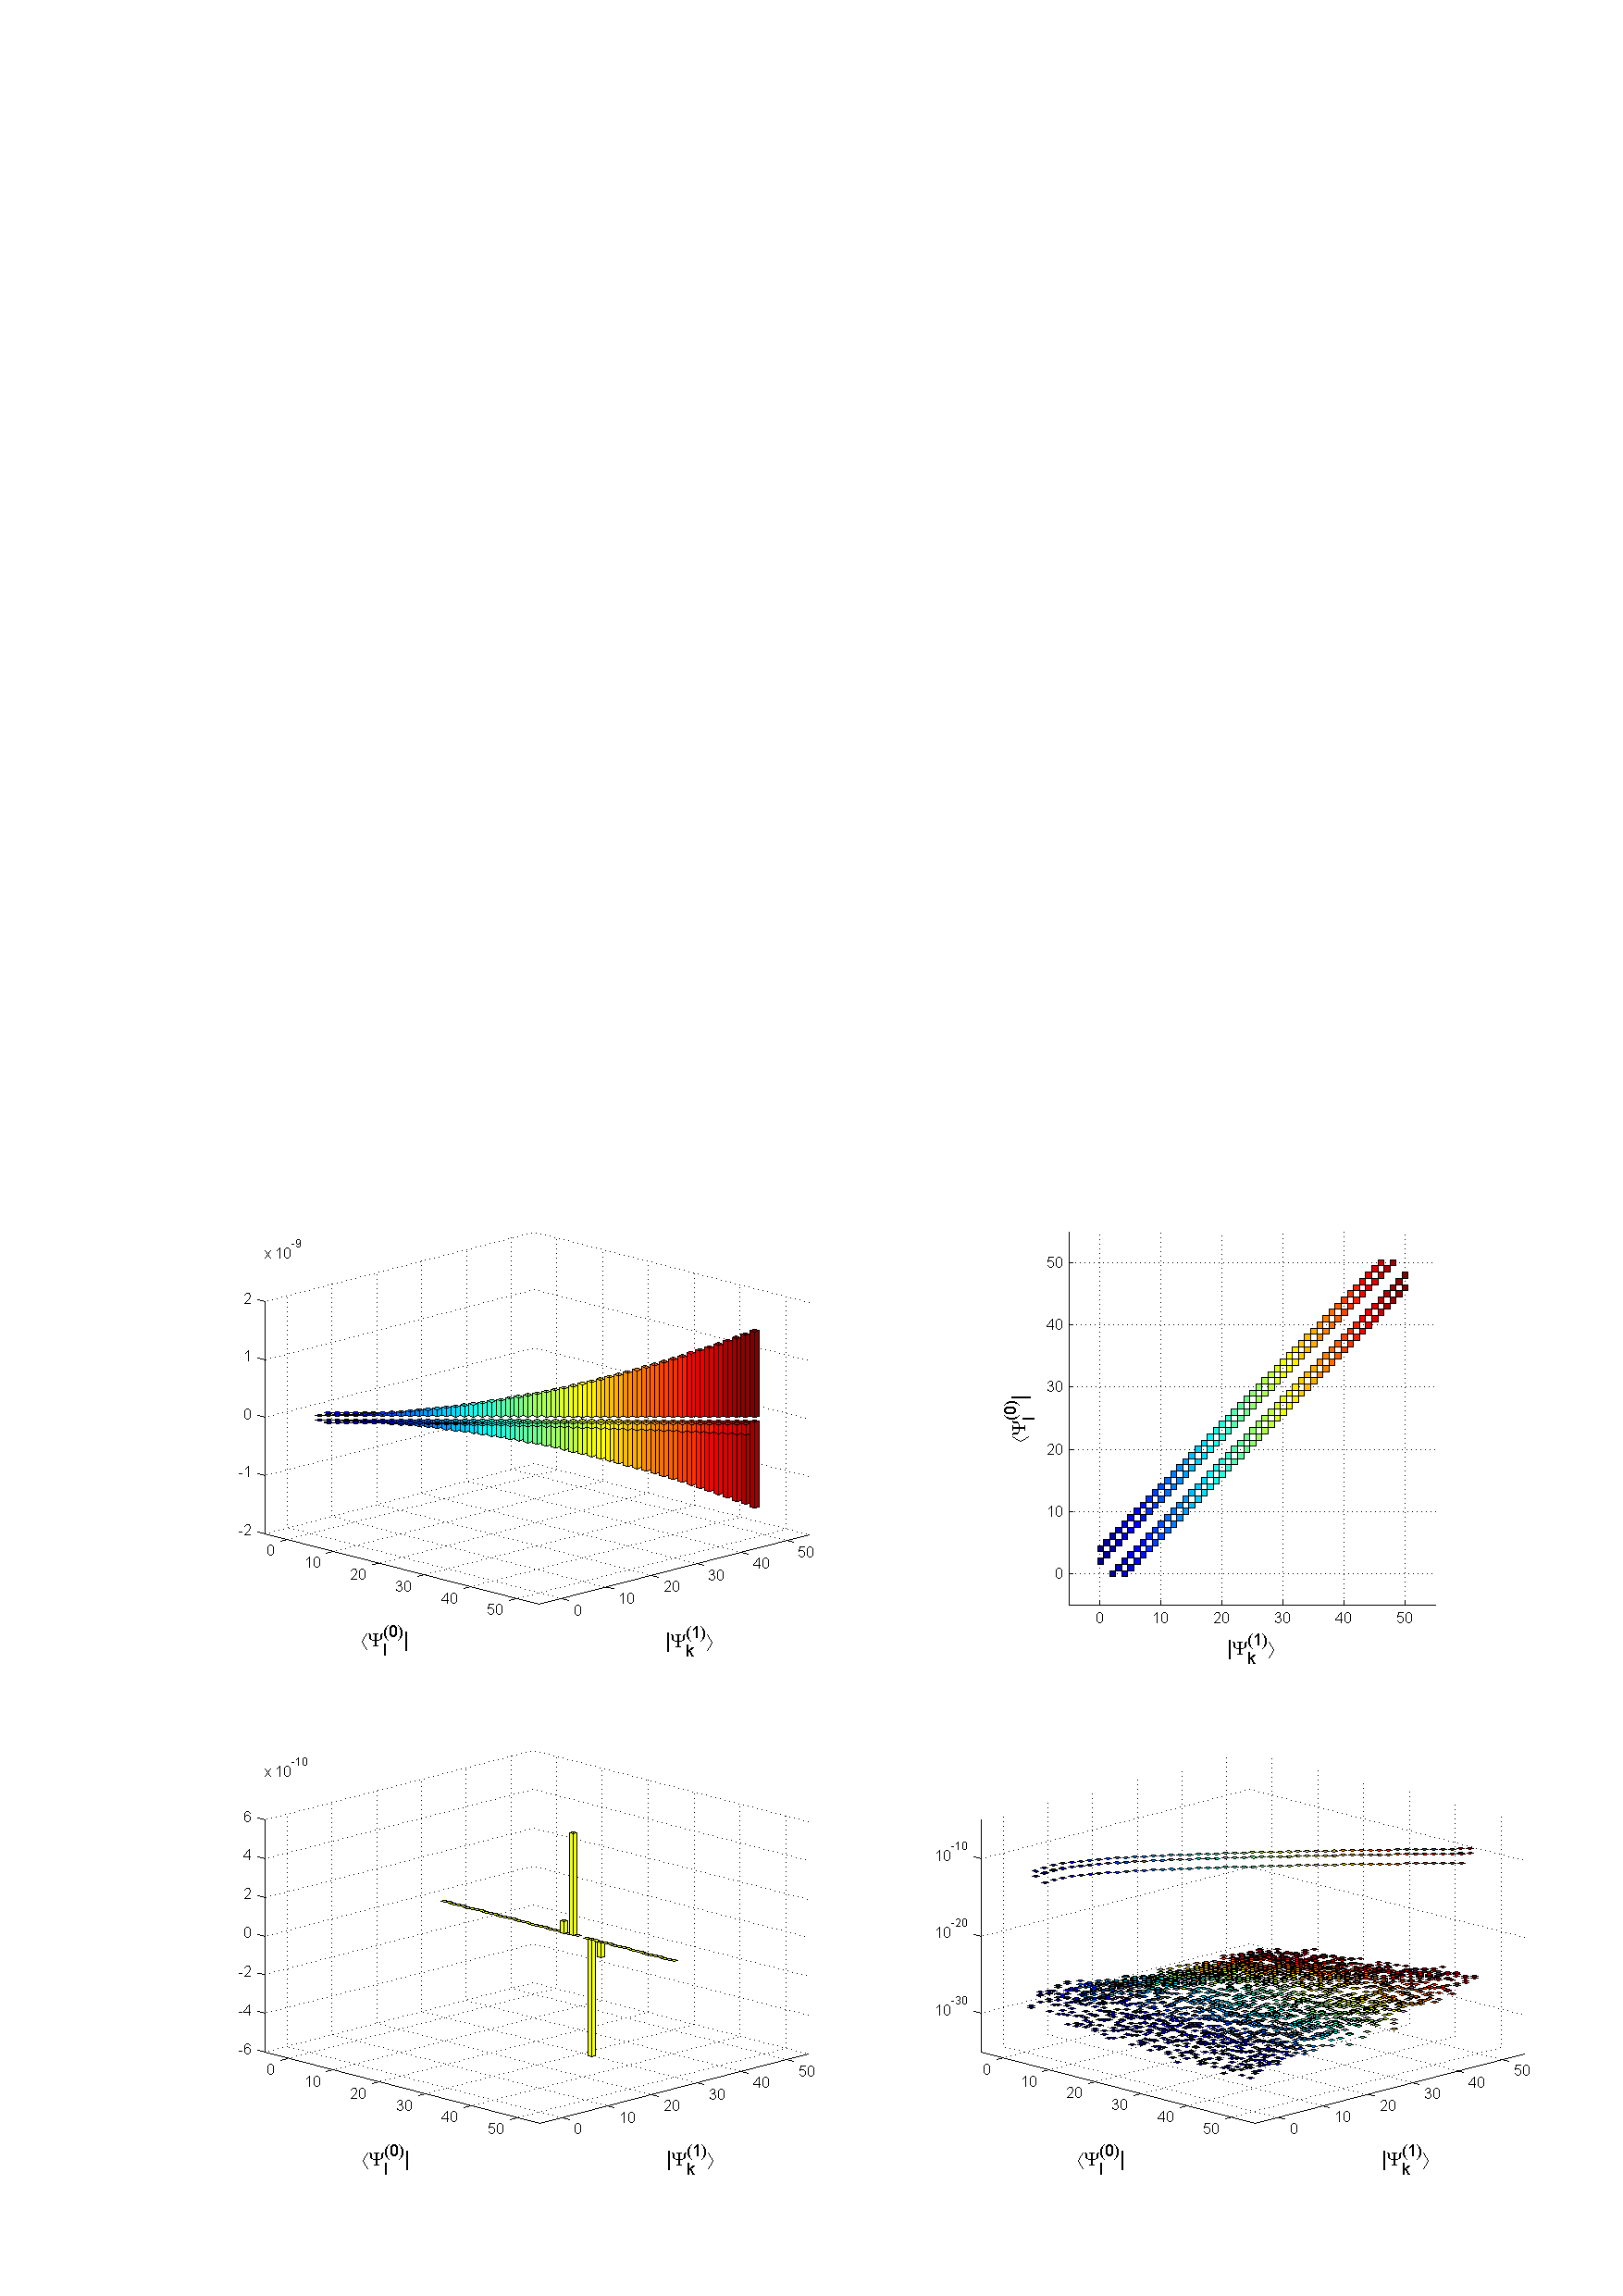
\includegraphics[width=1.0\textwidth]{anharmonisch/images/x4/Stoerung1Skalare.pdf}
\caption{Skalarprodukte $\langle\Psi_l^{(0)}|\Psi_k^{(1)}\rangle$ in erster N"aherung
\label{skript:x4_Stoerung1Skalare}}
\end{figure}

Auf der Abbildung~\ref{skript:x4_Stoerung1Skalare} sieht man welche ungest"orten Wellenfunktionen $\Psi_l^{(0)}$ den gr"ossten Anteil an der gest"orten Wellenfunktion $\Psi_k^{(1)}$ in erster N"aherung haben. Der Fall $k=l$ wird auf diesen Abbildungen nicht dargestellt. Wellenfunktionen, bei welchen $l=k\pm 1,k\pm 3,\dots$ ist, geben keinen Anteil an die gest"orte Wellenfunktion, da sie orthogonal dazu stehen. Ausserdem kann man sehen, dass bei gr"osseren $k$ auch die Anteile anderen Wellenfuntionen $l\neq k$ gr"osser werden. In der logarithmischen darstellung sieht man, dass die Wellenfuntionen, welche weiter weg sind nur noch einen vernachl"assigbar kleinen Beitrag liefern. Grunds"atzlich ist aber auch dort eine Zuhnahme bei den gr"osseren Wellenfunktionen zu erkennen.


\begin{figure}[h]	%Bild EK2.pdf
\centering
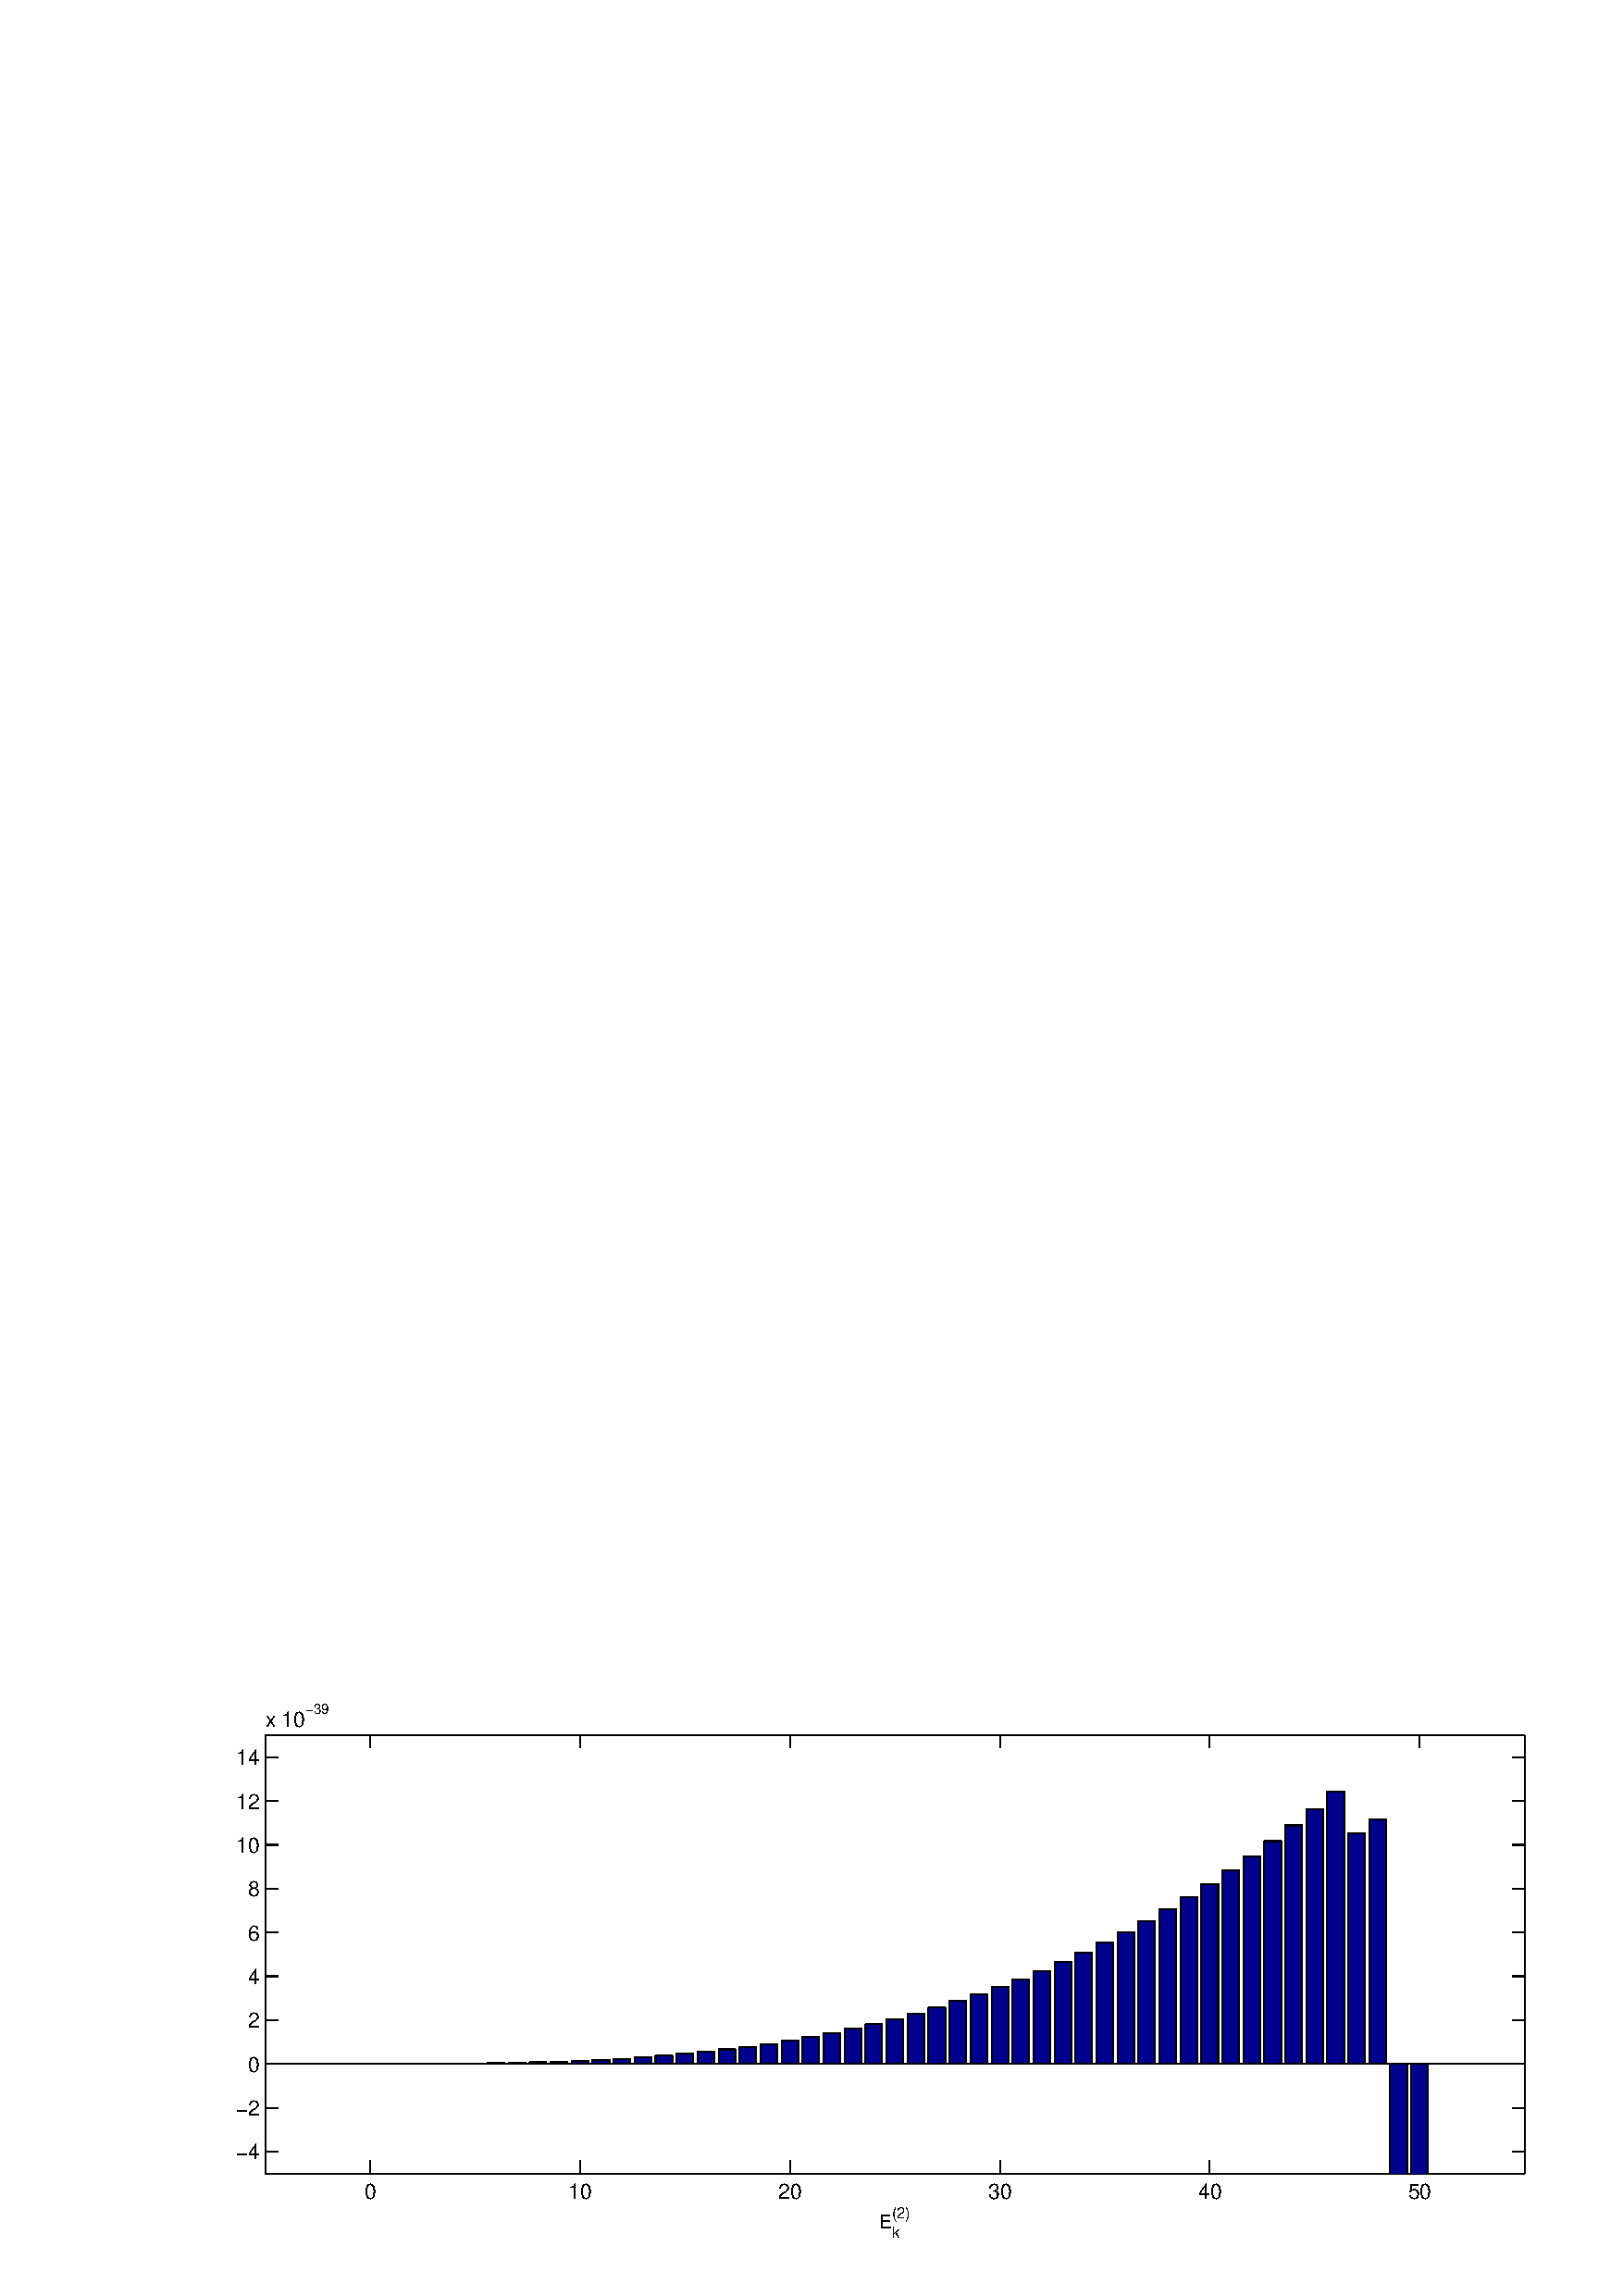
\includegraphics[width=0.6\textwidth]{anharmonisch/images/x4/EK2.pdf}
\caption{St"orung der Energieniveaus zweiter N"aherung
\label{skript:x4_EK2}}
\end{figure}

Auf der Abbildung~\ref{skript:x4_EK2} sieht man die "Anderung der Energieniveaus in zweiter N"aherung. Man kann klar Erkennen, dass die Abweichungen zum harmonischen Fall, bei h"oheren Energieniveaus immer gr"osser wird. Die Unstetigkeit bei den letzten drei Energieniveaus ist darauf zur"uckzuf"uhren, dass f"ur die Berechnung dieser Terme, Terme von Energieniveaus grösser 50 ben"otig werden, welche nicht mehr berechnet wurden.

\begin{figure}[h]	%Bild Stoerung2Wellenfunktion.pdf
\centering
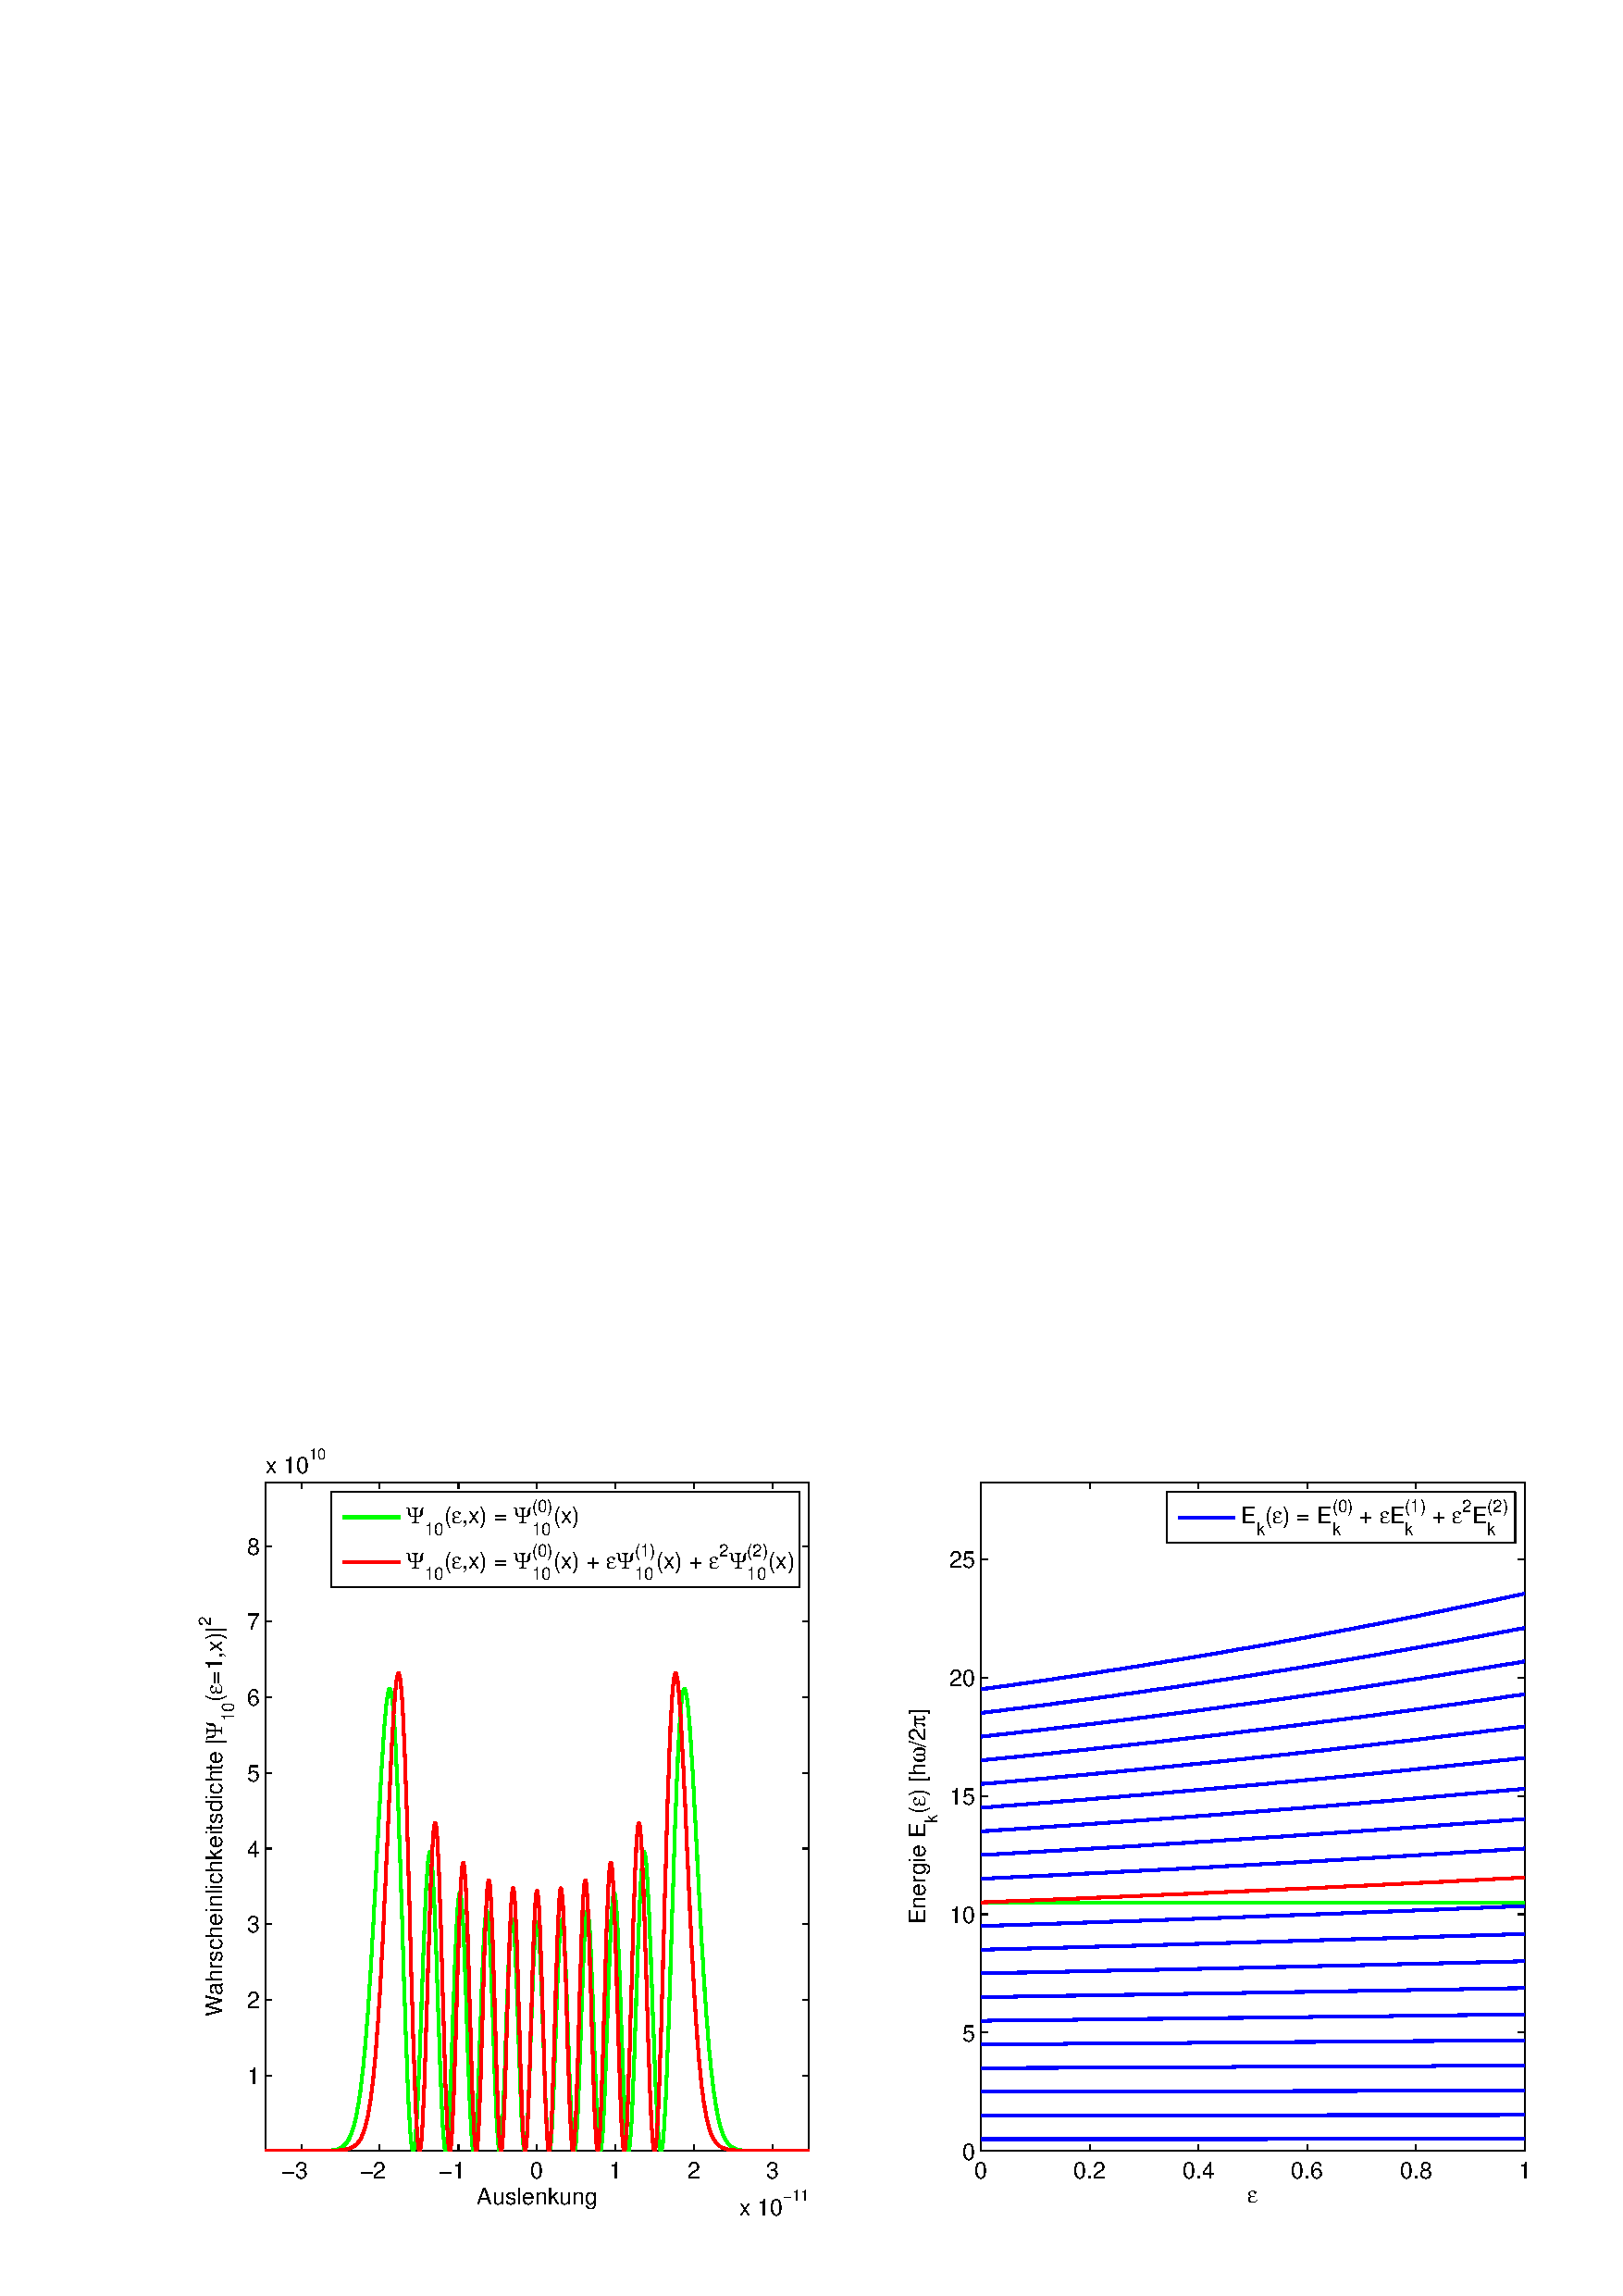
\includegraphics[width=0.8\textwidth]{anharmonisch/images/x4/Stoerung2Wellenfunktion.pdf}
\caption{10. Wellenfunktion und Energieniveaus in zweiter N"aherung
\label{skript:x4_Stoerung1Wellenfunktion}}
\end{figure}

Auf der Abbildung~\ref{skript:x4_Stoerung1Wellenfunktion} sieht man die 10. Wellenfunktion und die Energieniveaus in erster N"aherung. Man kann gut erkennen, dass sich die Energieniveaus nicht verschoben haben.

\begin{figure}[h]	%Bild Stoerung2Skalare.pdf
\centering
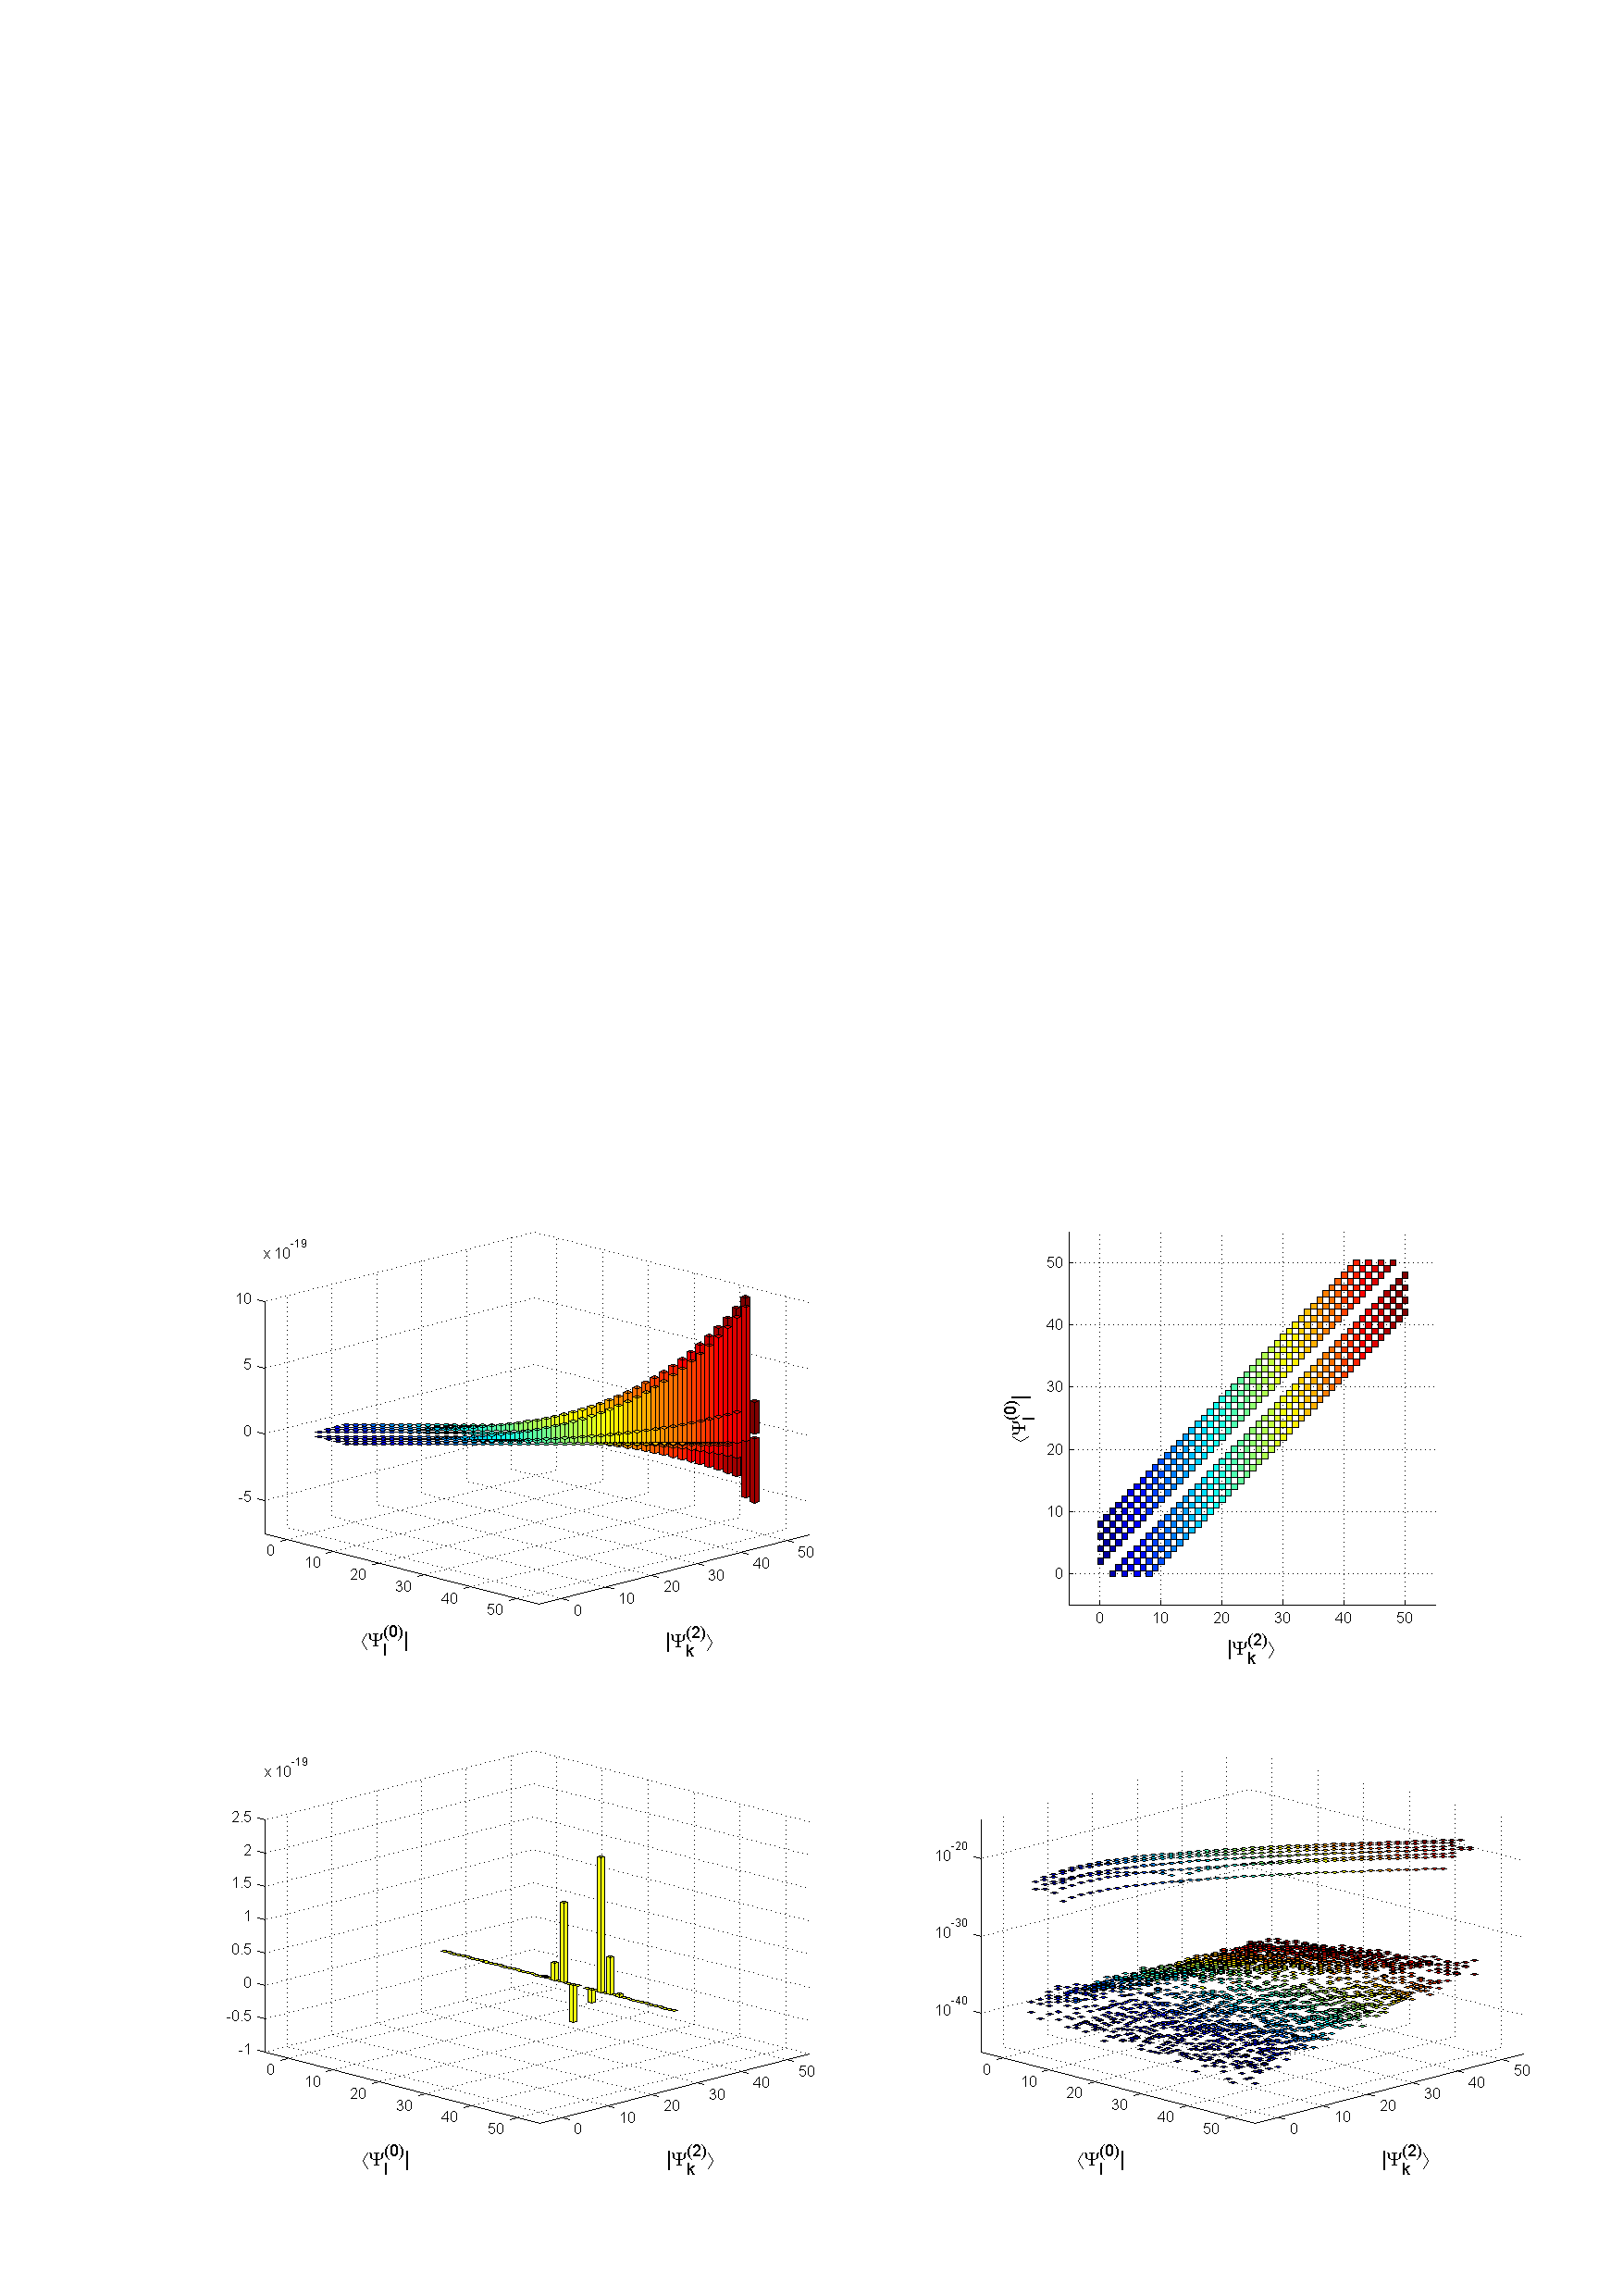
\includegraphics[width=1.0\textwidth]{anharmonisch/images/x4/Stoerung2Skalare.pdf}
\caption{Skalarprodukte $\langle\Psi_l^{(0)}|\Psi_k^{(2)}\rangle$ in zweiter N"aherung
\label{skript:x4_Stoerung2Skalare}}
\end{figure}

Auf der Abbildung~\ref{skript:x4_Stoerung1Skalare} sieht man welche ungest"orten Wellenfunktionen $\Psi_l^{(0)}$ den gr"ossten Anteil an der gest"orten Wellenfunktion $\Psi_k^{(2)}$ in zweiter N"aherung haben. Der Fall $k=l$ wird auf diesen Abbildungen nicht dargestellt. Wellenfunktionen, bei welchen $l=k\pm 1,k\pm 3,\dots$ ist, geben keinen Anteil an die gest"orte Wellenfunktion, da sie orthogonal dazu stehen. Ausserdem kann man sehen, dass bei gr"osseren $k$ auch die Anteile anderen Wellenfuntionen $l\neq k$ gr"osser werden. In der logarithmischen darstellung sieht man das die Wellenfuntionen, welche weiter weg sind nur noch einen vernachl"assigbar kleinen Beitrag liefern. Grunds"atzlich ist aber auch dort eine Zuhnahme bei den gr"osseren Wellenfunktionen zu erkennen.

\printbibliography[heading=subbibliography]
\end{refsection}

